% Se pre-carga la información del estudiante sólo para poder emplear el macro de
% selección de versión (digital o impresa)
% ===============================================================================
% El estudiante debe llenar sus datos en esta sección para que la plantilla los 
% auto-importe y genere automáticamente las páginas de portada y de firmas 
% autorizadas.
% ===============================================================================
% Datos del estudiante:
% -------------------------------------------------------------------------------
% Nombre completo
\def \nombreestudiante {Ángel Edgardo Orellana Sutuc}
% Carné
\def \uvgcarne {19095}
% Facultad
\def \uvgfacultad {Ingeniería}
% Carrera
\def \uvgcarrera {Ingeniería Electrónica}

% Datos del trabajo:
% -------------------------------------------------------------------------------
% Título completo
\def \titulotesis {Diseño e implementación de un sistema de carga multiquímica inteligente
para los agentes robóticos Pololu 3Pi+}
% Año de entrega
\def \anoentrega {2023}
% Asesor
\def \nombreasesor {Ing. Jonathan de los Santos}

% Datos del tribunal examinador:
% -------------------------------------------------------------------------------
% Nombre del primer examinador
\def \nombreprimerex {Msc. Miguel Zea}
% Nombre del segundo examinador
\def \nombresegundoex {Diego Morales}
% Año de aprobación
\def \anoaprobacion {2024}
% Mes de aprobación
\def \mesaprobacion {enero }
% Día de aprobación
\def \diaaprobacion {6 }

% Capítulos pre-definidos
% -------------------------------------------------------------------------------
% Comentar las líneas de las secciones que desean omitirse, por defecto se 
% se incluyen todas.
\def \CAPprefacio {Prefacio}
\def \CAPantecedentes {Antecedentes}
\def \CAPalcance {Alcance}
\def \CAPanexos {Anexos}
\def \CAPglosario {Glosario}

% Formato y estilo de la plantilla
% -------------------------------------------------------------------------------
% Modo impresión: Puede des-comentar la siguiente línea para generar un documento pdf sin la portada, para cuando se desee imprimir el documento para encuadernación
%\def \printver {Versión del documento para impresión}

% Portada: Puede cambiarse la imagen en la portada al cambiar el nombre del 
% archivo siguiente. NOTA: debe tener la suficiente resolución para cubrir el área
% designada
\def \imagenportada {plantilla/portadacit.jpg}

% Referencias: Puede des-comentar la siguiente línea para utilizar el formato de referencias APA
%\def \usarAPA {Usar formato APA}

% Párrafo: Puede comentar la siguiente línea si desea emplear un formato de 
% párrafo distinto al establecido por defecto
\def \parpordefecto {Formato de párrafo por defecto}

% Capítulos y secciones: Puede des-comentar la siguiente línea para establecer el
% formato de los capítulos y secciones bajo el estándar original de UVG para
% trabajos de graduación. Este incluye: capítulos con numeración romana, secciones
% con letras mayúsculas, sub-secciones con números y sub-sub-secciones con letras
% minúsculas
%\def \capsecuvg {Formato UVG para capítulos y secciones}

\ifdefined\printver
    \documentclass[11pt, letterpaper, twoside, openright]{report}
\else
    \documentclass[11pt, letterpaper]{report}
\fi

% Eliminar la opción de twoside y openright si se desea generar la versión
% digital del documento en lugar de la versión impresa
%\documentclass[11pt, letterpaper, twoside, openright]{report}
\usepackage[spanish, es-nodecimaldot, es-noquoting]{babel}
% cambiar a spanish, mexico si se quiere emplear tabla en lugar de cuadro
\selectlanguage{spanish}
\usepackage[utf8]{inputenc}
\usepackage[T1]{fontenc}

\title{Plantilla para Trabajos de Graduación IE-MT 2019v4}
\author{MSc. Miguel Zea}
\date{\today}

% Información del estudiante en el archivo datos_estudiante.tex
% ===============================================================================
% El estudiante debe llenar sus datos en esta sección para que la plantilla los 
% auto-importe y genere automáticamente las páginas de portada y de firmas 
% autorizadas.
% ===============================================================================
% Datos del estudiante:
% -------------------------------------------------------------------------------
% Nombre completo
\def \nombreestudiante {Ángel Edgardo Orellana Sutuc}
% Carné
\def \uvgcarne {19095}
% Facultad
\def \uvgfacultad {Ingeniería}
% Carrera
\def \uvgcarrera {Ingeniería Electrónica}

% Datos del trabajo:
% -------------------------------------------------------------------------------
% Título completo
\def \titulotesis {Diseño e implementación de un sistema de carga multiquímica inteligente
para los agentes robóticos Pololu 3Pi+}
% Año de entrega
\def \anoentrega {2023}
% Asesor
\def \nombreasesor {Ing. Jonathan de los Santos}

% Datos del tribunal examinador:
% -------------------------------------------------------------------------------
% Nombre del primer examinador
\def \nombreprimerex {Msc. Miguel Zea}
% Nombre del segundo examinador
\def \nombresegundoex {Diego Morales}
% Año de aprobación
\def \anoaprobacion {2024}
% Mes de aprobación
\def \mesaprobacion {enero }
% Día de aprobación
\def \diaaprobacion {6 }

% Capítulos pre-definidos
% -------------------------------------------------------------------------------
% Comentar las líneas de las secciones que desean omitirse, por defecto se 
% se incluyen todas.
\def \CAPprefacio {Prefacio}
\def \CAPantecedentes {Antecedentes}
\def \CAPalcance {Alcance}
\def \CAPanexos {Anexos}
\def \CAPglosario {Glosario}

% Formato y estilo de la plantilla
% -------------------------------------------------------------------------------
% Modo impresión: Puede des-comentar la siguiente línea para generar un documento pdf sin la portada, para cuando se desee imprimir el documento para encuadernación
%\def \printver {Versión del documento para impresión}

% Portada: Puede cambiarse la imagen en la portada al cambiar el nombre del 
% archivo siguiente. NOTA: debe tener la suficiente resolución para cubrir el área
% designada
\def \imagenportada {plantilla/portadacit.jpg}

% Referencias: Puede des-comentar la siguiente línea para utilizar el formato de referencias APA
%\def \usarAPA {Usar formato APA}

% Párrafo: Puede comentar la siguiente línea si desea emplear un formato de 
% párrafo distinto al establecido por defecto
\def \parpordefecto {Formato de párrafo por defecto}

% Capítulos y secciones: Puede des-comentar la siguiente línea para establecer el
% formato de los capítulos y secciones bajo el estándar original de UVG para
% trabajos de graduación. Este incluye: capítulos con numeración romana, secciones
% con letras mayúsculas, sub-secciones con números y sub-sub-secciones con letras
% minúsculas
%\def \capsecuvg {Formato UVG para capítulos y secciones}
% ================================================================================
% En este archivo se colocan opciones adicionales para modificar el formato de la
% plantilla, para emplearse en otros tipos de documentos que no sean trabajos de
% graduación. Si usted está trabajando su tesis, NO modifique este archivo
% ================================================================================
% Capítulos pre-definidos
% --------------------------------------------------------------------------------
% Comentar las líneas de las secciones que desean omitirse, por defecto se 
% se incluyen todas.
\def \CAPportada {Portada}
\def \CAPcaratula {Caratula}
\def \CAPfirmas {Hoja de firmas}
\def \CAPindice {Índice general}
\def \CAPfiguras {Listado de figuras}
\def \CAPcuadros {Listado de cuadros}
\def \CAPresumen {Resumen}
\def \CAPabstract {Resumen}
\def \CAPintroduccion {Introducción}
\def \CAPobjetivos {Objetivos}
\def \CAPjustificacion {Justificación}
\def \CAPmarcoteorico {Marco teórico}
\def \CAPconclusiones {Conclusiones}
\def \CAPrecomendaciones {Recomendaciones}
\def \CAPbibliografia {Bibliografía}

% ==============================================================================
% DEFINICIÓN DE PAQUETES
% ==============================================================================
\usepackage{xcolor}
\usepackage{amsfonts}
\usepackage{amsmath}
\usepackage{amssymb}
\usepackage{amsthm}
\usepackage{amsfonts}
\usepackage{mathtools}
\usepackage{graphicx}
\usepackage{xfrac}
\usepackage{float}
\usepackage{mathtools}
\usepackage[hypertexnames=false]{hyperref}
% \usepackage{bookmark}
\usepackage[font=small]{caption}
\usepackage{subcaption}
\usepackage{csquotes}
\usepackage{xpatch}
\usepackage{emptypage}
\usepackage{hyphenat}
\usepackage{fancyhdr}
\usepackage[backend=biber, style=ieee]{biblatex}
\addbibresource{m-bibliografias.bib}

\usepackage[percent]{overpic}

\usepackage{chngcntr}

\ifdefined\CAPglosario
	%\usepackage[toc]{glossaries}
	\usepackage[numberedsection]{glossaries}
	\makeglossaries
    \newglossaryentry{latex}
{
    name=latex,
    description={Es un lenguaje de marcado adecuado especialmente para la creación de documentos científicos}
} 
 
\newglossaryentry{formula}
{
    name=fórmula,
    description={Una expresión matemática} 
}
\fi

% ==============================================================================
% MÁRGENES Y FORMATO GENERALES
% ==============================================================================
\usepackage[top=1in, left=1.5in, right=1in, bottom=1in]{geometry}
%Options: Sonny, Lenny, Glenn, Conny, Rejne, Bjarne, Bjornstrup
\usepackage[Sonny]{fncychap}

% ==============================================================================
% DEFINICIONES DE LA PLANTILLA
% ==============================================================================
\graphicspath{ {figuras/} }
\definecolor{uvg-green}{RGB}{17,71,52}
\newcommand{\defaultparformat}[1]{
	{\setlength{\parskip}{2ex}
     \input{#1}}
}
\ifdefined\capsecuvg
	\renewcommand\thechapter{\Roman{chapter}}
    \renewcommand\thesection{\Alph{section}}
	\renewcommand\thesubsection{\arabic{subsection}}
    \renewcommand\thesubsubsection{\alph{subsubection}}
\fi
\counterwithout{figure}{chapter}
\counterwithout{table}{chapter}
\counterwithout{equation}{chapter}

\newcommand{\blankpage}{
\newpage
\thispagestyle{empty}
\mbox{}
\newpage
}
% ==============================================================================

% Comandos definidos por el usuario en el archivo comandos_usuario.tex
\usepackage{derivative}
\usepackage{pgfgantt}
\usepackage{xcolor,colortbl}
\usepackage{subcaption}
\usepackage{listings}
\usepackage{pdfpages}

\renewcommand\labelenumii{\theenumi.\arabic{enumii}.}
\renewcommand\labelenumiii{\theenumi.\theenumi.\arabic{enumii}.}

% Define colors for code highlighting
\definecolor{keywordcolor}{RGB}{0,0,255}
\definecolor{commentcolor}{RGB}{0,128,0}
\definecolor{stringcolor}{RGB}{255,0,0}
\definecolor{registercolor}{RGB}{128,0,128}

\lstdefinestyle{atmega328}{
    language=C,
    tabsize=1, 
    basicstyle=\fontsize{9}{12}\selectfont\ttfamily,
    keywordstyle=\color{keywordcolor},
    commentstyle=\color{commentcolor},
    stringstyle=\color{stringcolor},
    morekeywords={uint8_t,uint16_t,uint32_t},
    sensitive=false,
    morecomment=[l]{//},
    morecomment=[s]{/*}{*/},
    morestring=[b]",
    showstringspaces=false,
    breaklines=true,
    numbers=left,
    numberstyle=\tiny\color{gray},
    keywordstyle={[2]\color{registercolor}},
    keywords=[2]{DDRB, PORTB, PINB, DDRD, PORTD, PIND,TCCR0A,
                TCCR1A,TCCR2A,TCCR0B,TCCR1B,TCCR2B,OCR0A,OCR0B,
                OCR1A,OCR1B,OCR2A,OCR2B},
    emph={volatile},
    emphstyle=\textbf,
    literate=%
      {á}{{\'a}}1
      {é}{{\'e}}1
      {í}{{\'i}}1
      {ó}{{\'o}}1
      {ú}{{\'u}}1
      {Á}{{\'A}}1
      {É}{{\'E}}1
      {Í}{{\'I}}1
      {Ó}{{\'O}}1
      {Ú}{{\'U}}1
      {ñ}{{\~{n}}}1
      {Ñ}{{\~{N}}}1
}

\lstset{style=atmega328}

% ==============================================================================
% CUERPO DEL TRABAJO
% ==============================================================================
\pagestyle{headings}
\begin{document}

% ==============================================================================
% PORTADA
% ==============================================================================
\ifdefined\printver
    \let\CAPportada\undefined
\fi 

\ifdefined\CAPportada
    \cleardoublepage\phantomsection
    % \pdfbookmark{Portada}{toc}
	\newgeometry{left=3cm, bottom=0in, top=1in, right=3cm}
	\pagecolor{uvg-green}
	\thispagestyle{empty}

	\color{white}
	\noindent \hrulefill \par
	\vspace{0.1in}
	\noindent \Huge \nohyphens{\titulotesis} \par
	\noindent \hrulefill \par
	\noindent
	\LARGE \nombreestudiante

	\begin{figure}[b!]
    	%\makebox[\textwidth]{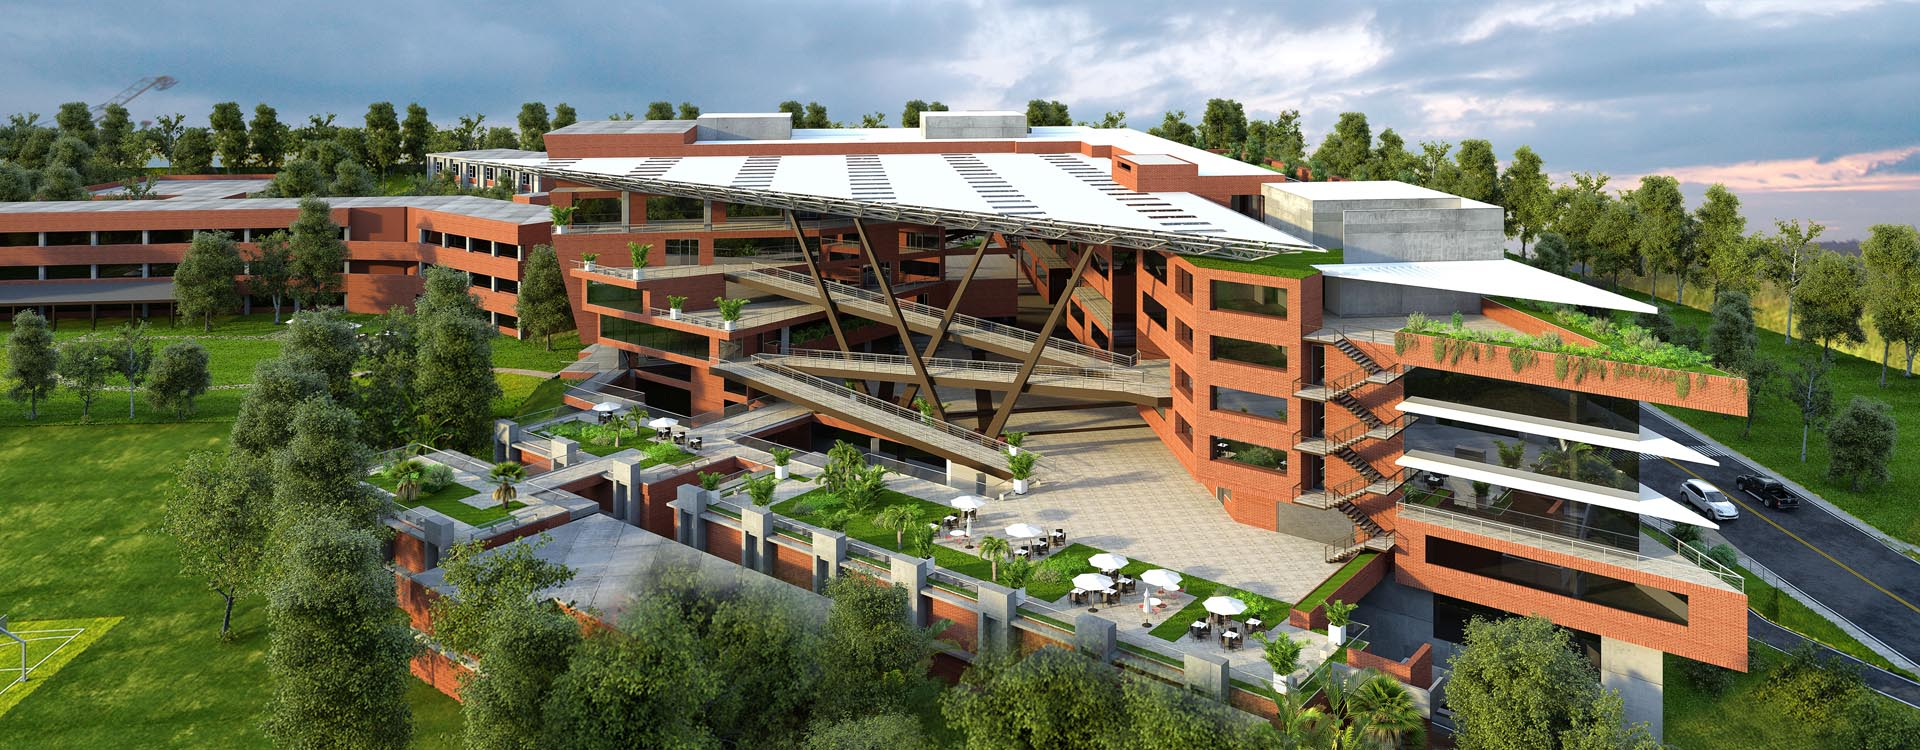
\includegraphics[height=13.25cm]{plantilla/portadacit.jpg}}
    	\makebox[\textwidth]{
    		\begin{overpic}[height=13.25cm]{\imagenportada}
     		\put(63,0){
\includegraphics[height=1.15in]{plantilla/fondologo_grande.png}}  
  			\put(64.5,2){
\includegraphics[height=0.55in]{plantilla/logoUVGblanco.eps}} 
        	\end{overpic}
    	}
    	%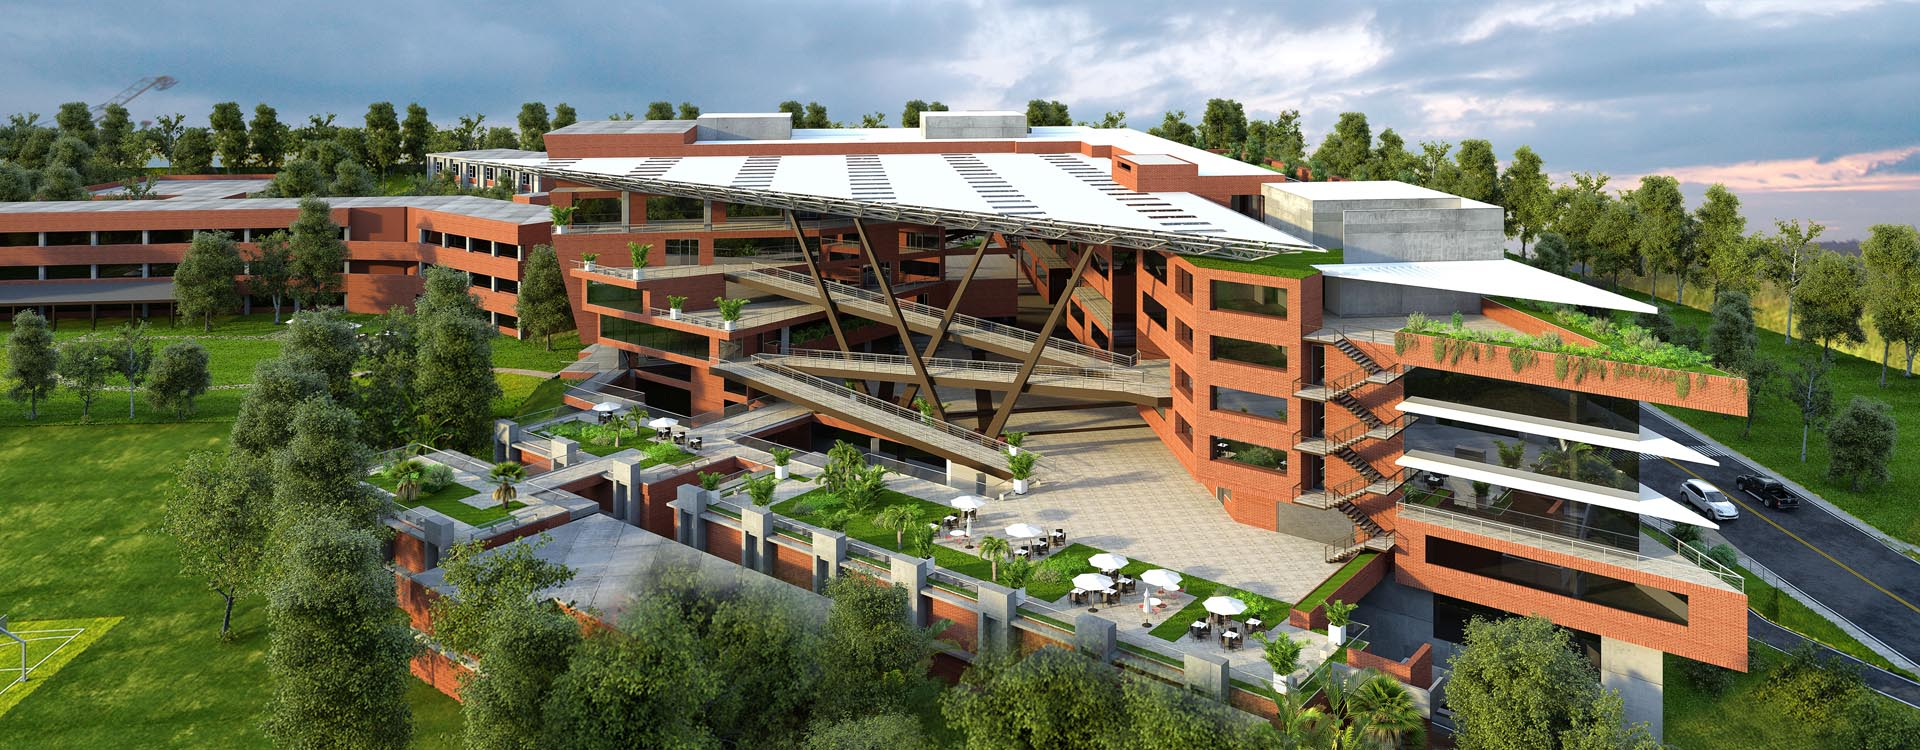
\includegraphics[height=13.25cm]{plantilla/portadacit.jpg}
	\end{figure}
	\restoregeometry
\fi

% ==============================================================================
% PRIMERAS PÁGINAS (Carátulas más hojas de guarda)
% ==============================================================================
\ifdefined\CAPcaratula
	\newpage
    \cleardoublepage\phantomsection
    % \pdfbookmark{Carátula}{toc}
	\pagecolor{white}
	\color{black}
	\setcounter{page}{1}
	\pagenumbering{roman}
	\thispagestyle{empty}
	\begin{center}
		\LARGE UNIVERSIDAD DEL VALLE DE GUATEMALA\\
		\LARGE Facultad de \uvgfacultad \\[0.75cm]
	\end{center}
	\begin{figure}[h]
		\begin{center}
		
\includegraphics[height=5.5 cm]{plantilla/escudoUVGnegro.eps}
		\vspace{0.5in}
		\end{center}
	\end{figure}
	\begin{center}
		\Large \textbf{\nohyphens{\titulotesis}} \\
		%\LARGE \textbf{\titulotesis} \\
		\vfill
		\Large \nohyphens{Trabajo de graduación presentado por \nombreestudiante \ para optar al grado académico de Licenciado en \uvgcarrera} \\
		\vfill
		\large Guatemala, \\
		\vspace{1em}
		\anoentrega
	\end{center}
    
    \ifdefined\printver	
	    \blankpage
	    \blankpage
	    
	    \newpage
	    \cleardoublepage\phantomsection
	    \pagecolor{white}
    	\color{black}
    	\setcounter{page}{1}
    	\pagenumbering{roman}
    	\thispagestyle{empty}
    	\begin{center}
    		\LARGE UNIVERSIDAD DEL VALLE DE GUATEMALA\\
    		\LARGE Facultad de \uvgfacultad \\[0.75cm]
    	\end{center}
    	\begin{figure}[h]
    		\begin{center}
    		
\includegraphics[height=5.5 cm]{plantilla/escudoUVGnegro.eps}
    		\vspace{0.5in}
    		\end{center}
    	\end{figure}
    	\begin{center}
    		\Large \textbf{\nohyphens{\titulotesis}} \\
    		%\LARGE \textbf{\titulotesis} \\
    		\vfill
    		\Large \nohyphens{Trabajo de graduación presentado por \nombreestudiante \ para optar al grado académico de Licenciado en \uvgcarrera} \\
    		\vfill
    		\large Guatemala, \\
    		\vspace{1em}
    		\anoentrega
    	\end{center}
    \fi
\fi

% ==============================================================================
% HOJA DE FIRMAS
% ==============================================================================
\ifdefined\CAPfirmas
	\newpage
	\cleardoublepage\phantomsection
	\thispagestyle{empty}
	\vspace*{0.5in}
	\large Vo.Bo.:\\[1cm]
	\begin{center}
		(f) \rule[1pt]{4 in}{1pt}\\
		\nombreasesor
	\end{center}
	\vspace{1in}

	Tribunal Examinador:\\[1cm]
	\begin{center}
		(f) \rule[1pt]{4 in}{1pt}\\
		\nombreasesor \\[1in]
		(f) \rule[1pt]{4 in}{1pt}\\
		\nombreprimerex \\[1in]
		(f) \rule[1pt]{4 in}{1pt}\\
		\nombresegundoex
	\end{center}
	\vspace{1in}

%	Fecha de aprobación: Guatemala, \rule[1pt]{0.5 in}{1pt} de \rule[1pt]{1 in}{1pt} de \anoaprobacion.
    Fecha de aprobación: Guatemala, \mesaprobacion de \anoaprobacion. %\diaaprobacion de \mesaprobacion de \anoaprobacion.
	\normalsize
\fi

% Comentar para formato estilo libro en la numeración de páginas (NO 
% compatible con la guía UVG 2019)
\pagestyle{plain}
% ==============================================================================
% CONTENIDO DEL TRABAJO
% ==============================================================================
% PREFACIO
% ------------------------------------------------------------------------------
\ifdefined\CAPprefacio
	\newpage
	\cleardoublepage\phantomsection
    \chapter*{Prefacio}
    \ifdefined\parpordefecto
    	\defaultparformat{a-prefacio}
    \else
    	Quiero comenzar este trabajo de graduación expresando mi agradecimiento a
quienes han sido fundamentales en mi carrera académica. A mi familia, por su
amor, sacrificio y apoyo constante a lo largo de este camino. A mi querida
novia, Janny Garcia, por su apoyo y consejos invaluables en los momentos
difíciles. A mis amigos, en especial a Daniel Mundo, Noel Prado, Julio
Lopez, Victor Vanegas, Angelo Machorro y Saúl de León, por su amistad y aliento
inquebrantable. Este trabajo de graduación es el resultado de años de esfuerzo 
y dedicación, y cada uno de ustedes ha tenido un papel importante en mi camino 
hacia la culminación de esta etapa académica. Finalmente, quiero agradecer a mi
universidad, a mis profesores y a todos aquellos que contribuyeron a mi 
formación académica. Con gratitud, les dedico este trabajo como una muestra
 de mi aprecio y reconocimiento por su apoyo continuo.

 
    \fi
    \addcontentsline{toc}{chapter}{Prefacio}
\fi

% ÍNDICE GENERAL
% ------------------------------------------------------------------------------
\ifdefined\CAPindice
	\newpage
    \cleardoublepage\phantomsection
	\renewcommand{\contentsname}{Índice}
    %\phantomsection
    \pdfbookmark{\contentsname}{toc}
    %\pdfbookmark{Índice}{toc}
	\tableofcontents
\fi

% LISTADO DE FIGURAS
% ------------------------------------------------------------------------------
\ifdefined\CAPfiguras
	\newpage
    \cleardoublepage\phantomsection
	\renewcommand{\listfigurename}{Lista de figuras}
	\listoffigures
	\addcontentsline{toc}{chapter}{Lista de figuras}
\fi

% LISTADO DE CUADROS
% ------------------------------------------------------------------------------
\ifdefined\CAPcuadros
	\newpage
    \cleardoublepage\phantomsection
	\renewcommand{\listtablename}{Lista de cuadros}
	\listoftables
	\addcontentsline{toc}{chapter}{Lista de cuadros}
\fi

% RESUMEN
% ------------------------------------------------------------------------------
\ifdefined\CAPresumen
	\newpage
    \cleardoublepage\phantomsection
	\chapter*{Resumen}
	\ifdefined\parpordefecto
		\defaultparformat{b-resumen}
	\else
		Este proyecto se centra en el desarrollo de un sistema de carga multiquímica para baterías NiMH y Li-ion.
Para ello fue necesario el diseño de  una fuente de corriente/voltaje constante 
la cual es  controlada mediante una señal analógica de voltaje.

Para medir la corriente entregada a las baterías (cuando se opera en modo de
corriente constante), se implementó un sensor utilizando el amplificador
operacional TL082 en configuración amplificador diferencial, 
junto con una resistencia shunt de $15 \text{m}\Omega$ para la conversión de corriente a
voltaje.

Además, se diseñó un conversor digital a analógico que utiliza
uno de los dos amplificadores operacionales del TL082 en configuración seguidor
en conjunto con un filtro RC con una frecuencia de corte de 72.3 Hz para filtrar
los armónicos de una señal PWM, de forma que únicamente se tenga a la salida la
componente DC de la señal PWM.

Para la carga de las baterías NiMH se ha implementado el algoritmo de carga 
denominado \textit{trickle charge} el cual consiste en cargar las baterías
a una corriente constante de valor bajo (para este casó 0.1C) hasta que las
baterías alcancen su voltaje nominal, el cual es de 6V. Para la carga de las baterías 
Li-ion se ha implementado el algoritmo de carga
denominado carga por corriente constante-voltaje constante, deteniendo el proceso
de carga cuando la corriente entregada a la batería es menor al 10\% de la capacidad
de la batería.


Se diseñó un multiplexor de potencia con el propósito de gestionar
la carga de las baterías NiMH y
Li-ion, de forma que ambas baterías puedan ser recargadas con un único convertidor
reductor. Además, se ha incorporado otro multiplexor 
de potencia para determinar que batería está proporcionando potencia al 
agente robótico Pololu 3pi+. Adicionalmente se desarrolló una estación de carga que cuenta con conectores USB-A
hembra para suministrar 12 V a la placa de expansión del agente robótico Pololu 3Pi+.



	\fi
	\addcontentsline{toc}{chapter}{Resumen}
\fi

% ABSTRACT
% ------------------------------------------------------------------------------
\ifdefined\CAPabstract
	\newpage
    \cleardoublepage\phantomsection
	\chapter*{Abstract}
	\ifdefined\parpordefecto
		\defaultparformat{c-abstract}
	\else
		This project focuses on the development of a multi-chemistry charging system for
NiMH and Li-ion batteries. To achieve this, it was necessary to design a 
constant current/voltage source controlled by an analog voltage signal.

To measure the current delivered to the batteries (when operating in constant
current mode), a sensor has been implemented using the TL082 operational 
amplifier in a differential amplifier configuration, along with a $15 \text{m}\Omega$ shunt resistor for current-to-voltage conversion.

Furthermore, a digital-to-analog converter (DAC) has been designed using one of the two operational amplifiers in the TL082, configured as a voltage follower, in conjunction with an RC filter with a cutoff frequency of 72.3 Hz to filter out the harmonics of a PWM signal, allowing only the DC component of the PWM signal to pass through.

For charging NiMH batteries, the charge algorithm known as "negative voltage change"  has been implemented. This algorithm involves detecting a negative change in battery voltage, indicating that the battery is fully charged. For Li-ion battery charging, the "constant current-constant voltage" charge algorithm has been implemented, with the charging process stopping when the current delivered to the battery drops below 10% of the battery's capacity.

A power multiplexer has been implemented to switch the power source from NiMH to Li-ion batteries to the charging system, enabling one battery to be charged at a time. Additionally, a power multiplexer has been implemented to determine which battery is connected to the 3pi+ robot.

The charging system includes a station with female USB A connectors to supply 12V to the Pololu 3Pi+ robot's expansion board and allow the passage of UART communication lines from the microcontroller via a magnetic USB cable.
	\fi
	\addcontentsline{toc}{chapter}{Abstract}
\fi

% INTRODUCCIÓN
% ------------------------------------------------------------------------------
\ifdefined\CAPintroduccion
	\newpage
	\cleardoublepage
	\pagenumbering{arabic}
	\setcounter{page}{1}
	\chapter{Introducción}
	\ifdefined\parpordefecto
		\defaultparformat{d-introduccion}
	\else
		% necesito redactar la introduccion de mi tesis

En el ámbito de la robótica, y más específicamente en el campo de
 la robótica de enjambres, la autonomía de los agentes robóticos emerge como
un elemento fundamental. La mejora de esta autonomía requiere que estos agentes
estén equipados con sistemas de alimentación que les permitan operar durante 
períodos prolongados sin intervención humana. Para alcanzar este objetivo, es 
necesario que estos agentes dispongan de sistemas de carga que les permitan 
recargar sus baterías de manera autónoma.

En el caso de los agentes robóticos Pololu 3Pi+, se caracterizan por contar
con un banco de baterías NiMH compuesto por 4 celdas en serie, que son 
recargables. No obstante, carecen de un sistema de carga incorporado, lo 
que obliga a extraer las baterías para su recarga.

El presente trabajo se enfoca en diseño y construcción de un sistema 
de carga multiquímica diseñado específicamente para las baterías NiMH y 
Li-ion utilizadas en los agentes robóticos Pololu 3Pi+. Este sistema de carga 
tiene como propósito habilitar la recarga del banco de baterías NiMH sin 
requerir la extracción de las mismas. Además, se introduce una batería de 
respaldo Li-ion 18650 con el fin de ampliar la autonomía de los agentes 
robóticos y brindar energía adicional para alimentar módulos auxiliares.

Como componente esencial del sistema de carga, se han desarrollado estaciones
de carga magnéticas. Estas estaciones permiten que los agentes Pololu 3Pi+ 
identifiquen niveles bajos de carga y acudan automáticamente a la estación más cercana para recargar ambas baterías.

	\fi
\fi

% ANTECEDENTES
% ------------------------------------------------------------------------------
\ifdefined\CAPantecedentes
	\newpage
	\chapter{Antecedentes}
	\ifdefined\parpordefecto
    	\defaultparformat{e-antecedentes}
    \else
    	\section{Robotat}

En la Universidad del Valle de Guatemala se cuenta con el ecosistema Robotat descrito
 en \cite{perafan_montoya_robotat_2022}, que consiste en un ecosistema formado por una red
 de comunicación WiFi, así como también un sistema de captura de movimiento OptiTrack, el 
 cual emplea un total de seis cámaras. Adicionalmente Robotat cuenta con una antena inteligente la cual
 combina la información obtenida por medio del sistema de captura de movimiento, con información dada
 por una unidad de medición inercial de forma que es posible el intercambio de información entre agentes
 mediante comunicación inalámbrica.

\begin{figure}[H]
        \centering
        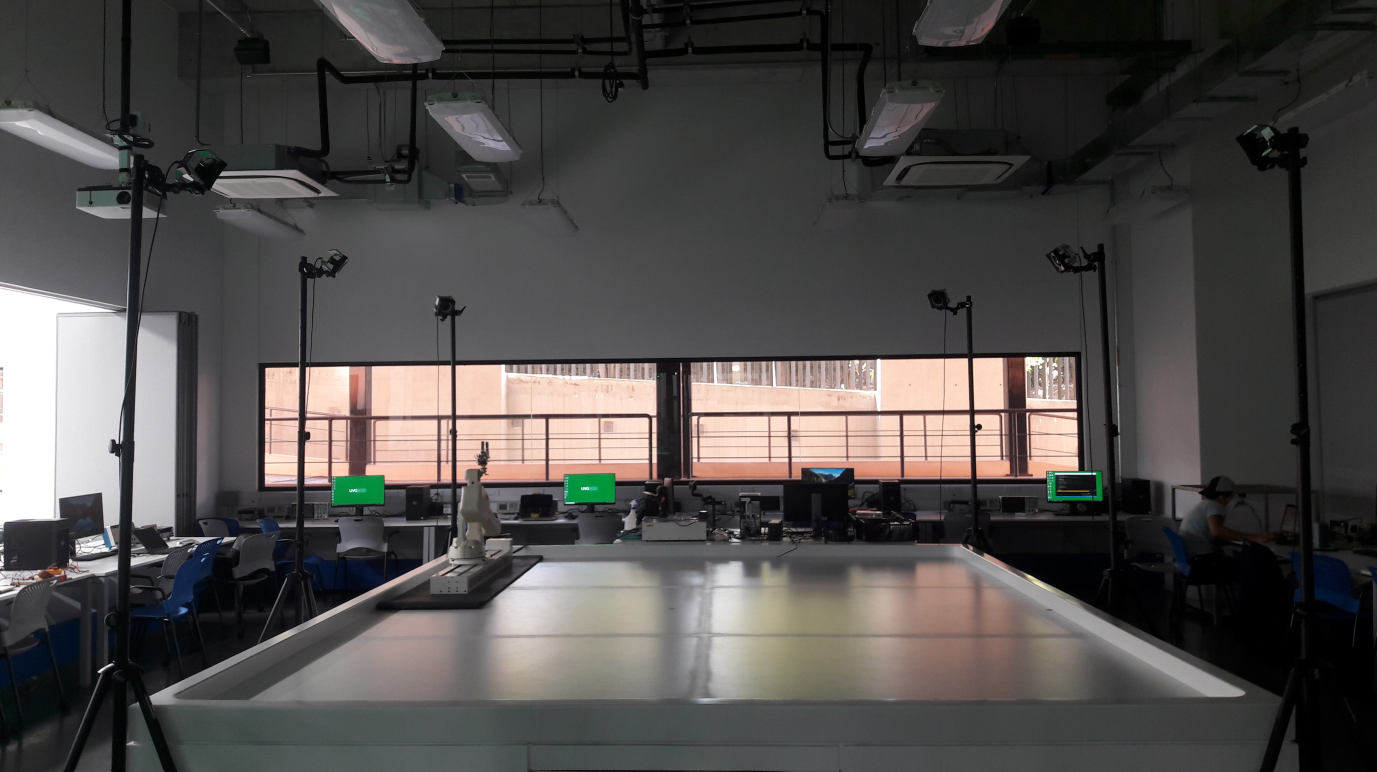
\includegraphics[scale=.4]{imagenes/robotat.png}
        \caption{Ecosistema Robotat \cite{perafan_montoya_robotat_2022}}
        \label{fig:robotat}
\end{figure}

\section{Robotarium del Georgia Institute of Technology}

El Robotarium es un proyecto diseñado por \textit{Georgia Institute of Technology}, con la finalidad
de tener una plataforma \textit{multi-robot} que pueda ser accedida de forma remota y de fácil acceso al público.

Este proyecto es presentado en \cite{wilson_robotarium_2021} como una herramienta de propósitos educacionales
así como para aplicaciones de robótica avanzada. 
En el prototipo inicial del Robotarium, los agentes robóticos utilizados son
GRITSBot que, para asegurar su autonomía se encontraban equipados con un sistema de carga inalámbrica,
 el cual tenía bobinas de inducción orientadas hacia el suelo
de forma que los GRITSBot eran recargados por medio de transmisores instalados en el suelo. Sin embargo, este sistema
contaba con la desventaja que para maximizar la eficiencia al cargar,  era necesario que los 
transmisores y las bobinas instaladas en los agentes estuvieran lo más cerca posible. Debido a las técnicas
 de fabricación existía la posibilidad de que los robots montados se arrastraran en la superficie,
o bien se encontrarían a una distancia que impidiera la carga.

Debido a los inconvenientes mencionados anteriormente el sistema de carga fue reemplazado por unidades de transmisión
inalámbricas colocadas en los muros de la arena del Robotarium, así como también unidades receptoras instaladas en la 
parte trasera de los GRITSbot. Con este nuevo diseño las unidades de carga pueden ser manufacturadas de forma
 mas rápida, utilizando corte láser, y cargadores inalámbricos comerciales. Adicionalmente al estar los cargadores
 montados en el muro se tiene un proceso de carga más fiable al permitir un contacto casi directo con los robots,
 sin la necesidad de colocar los receptores cerca del suelo \cite{wilson_robotarium_2021}. 

 \begin{figure}[H]
    \centering
    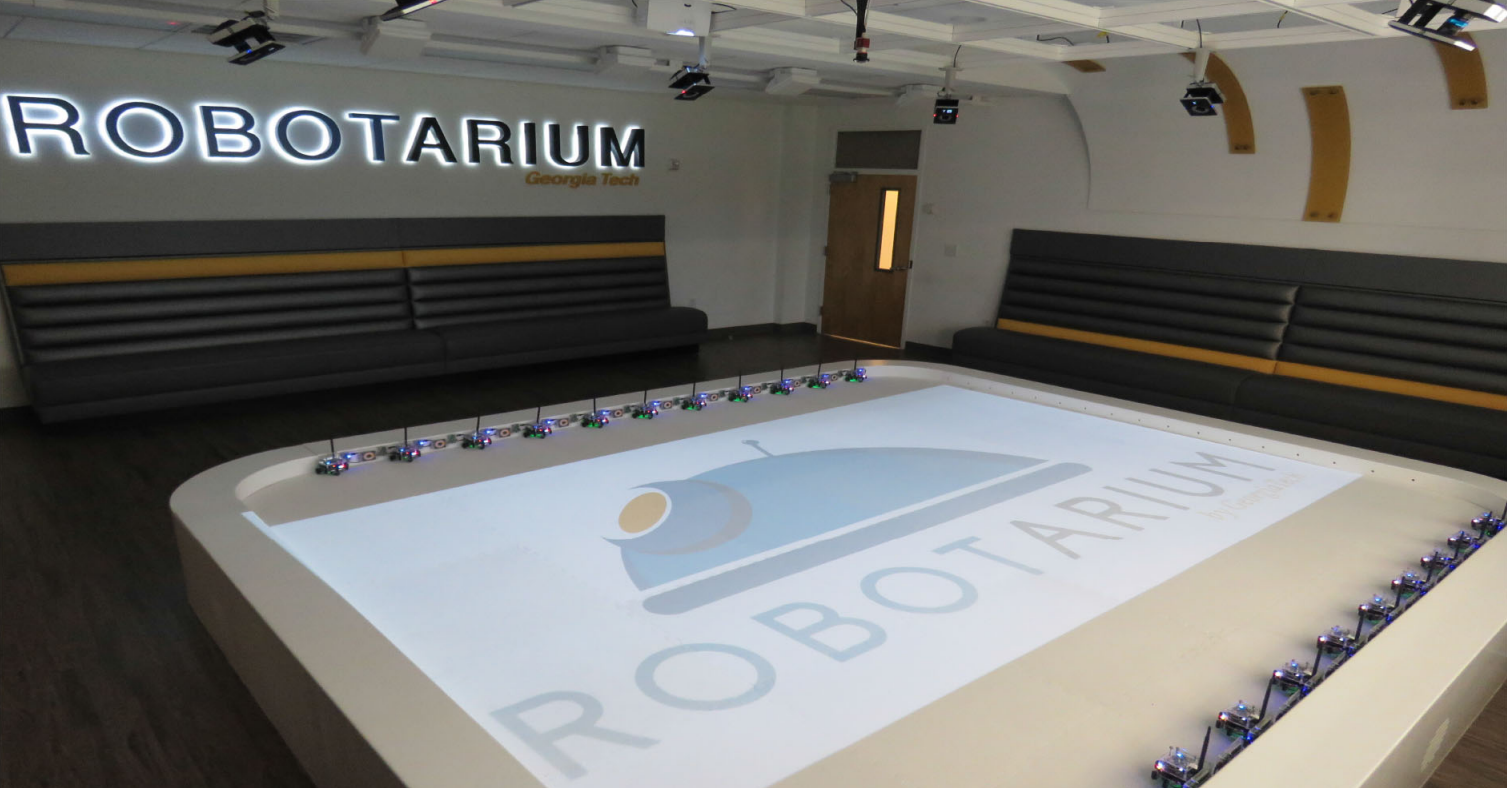
\includegraphics[scale=.4]{imagenes/Robotarium.png}
    \caption{Arena del  Robotarium  \cite{wilson_robotarium_2021}}
    \label{fig:robotarium}
\end{figure}

\section{Cargadores de baterías multiquímica}
En la actualidad para muchas aplicaciones es de gran importancia el uso
baterías para tener movilidad y autonomía, de igual forma también es indispensable
el desarrollo de sistemas de carga que sean eficientes. En \cite{cleveland_developing_2015}
se presenta el desarrollo de un cargador multiquímica de baterías programable, el cual se 
encuentra basado en el circuito integrado MCP19111 de Microchip, que es un
\textit{Digitally-Enhanced Power Analog Controller}, este, a grandes rasgos es un controlador el cual
contiene lazos de control analógicos con interfaces digitales para el monitoreo y manipulación de parámetros
de forma que sea posible el ajuste del sistema mientras se encuentra en operación pudiendo mejorar el rendimiento
significativamente.  

En el \textit{Massachusetts Institute of Technology} se desarrolló el sistema WafferSat el cual  es un satélite que emplea 
sistemas microelectromecánicos para reducir su tamaño. En \cite{zapien_electrical_2020} se explica el uso del controlador de 
carga BQ25703A, manufacturado por Texas Instruments para el diseño de seguidor de máximo punto de potencia (MPPT, por
sus siglas en inglés) el cual es empleado en el WafferSat para el sistema de carga solar de baterías de polímero
 de iones de litio (LiPo).

\section{Estación de carga inalámbrica para UAV}

En \cite{junaid_design_2016}, se presenta el diseño de una estación de carga inalámbrica para UAV
(Vehículo Aéreo No Tripulado, por sus siglas en inglés). Este proyecto surge debido a que los multicópteros,
 en general, tienen una demanda alta de potencia, lo que limita su tiempo de vuelo, especialmente en el caso
de aquellos de pequeñas dimensiones. Para lograr que estos multicópteros puedan operar durante períodos prolongados,
resulta necesario recargar sus baterías, lo cual generalmente requiere intervención humana directa. En el desarrollo
de esta plataforma de carga, se utilizó la placa DFRobot Leonardo, basada en el microcontrolador ATmega32u4, que
incluye un conector Xbee integrado para permitir la comunicación inalámbrica con módulos Zigbee. En cuanto a la transmisión
de energía hacia el multicóptero, se empleó un sistema de carga inalámbrica, el cual fue prototipado utilizando placas perforadas.
 El sistema diseñado logró alcanzar una eficiencia máxima del 63.4\% \cite{junaid_design_2016}.

\begin{figure}[H]
    \centering
    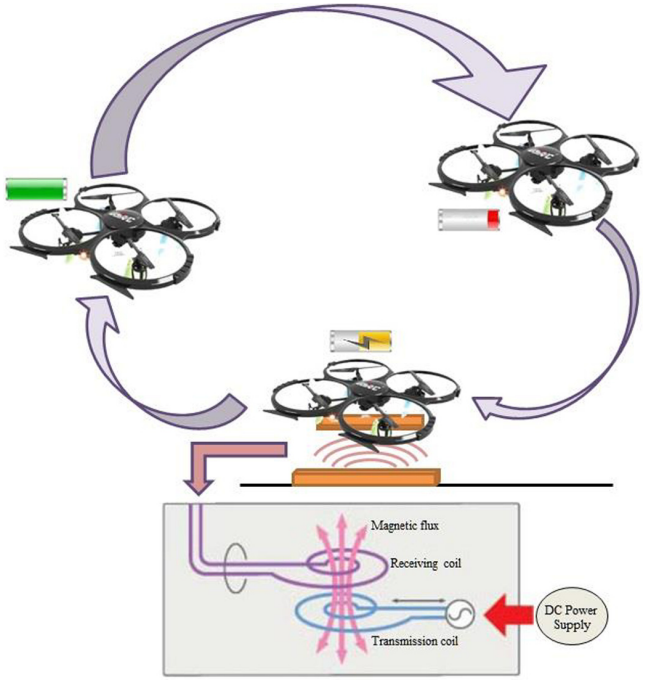
\includegraphics[scale=.4]{imagenes/AUV.png}
    \caption{Concepto de la solución propuesta \cite{junaid_design_2016}}
    \label{fig:1}
\end{figure}

\begin{figure}[H]
    \centering
    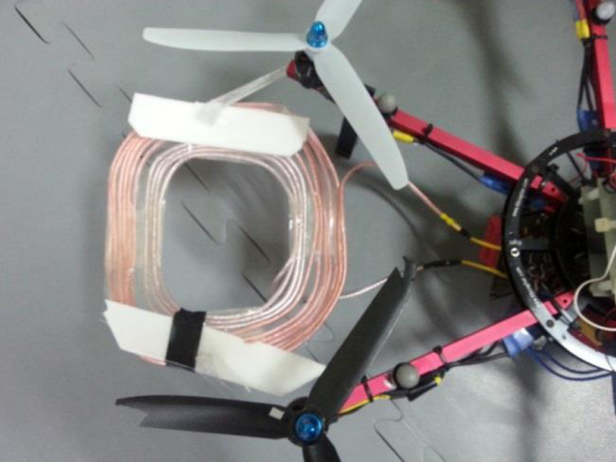
\includegraphics[scale=.4]{imagenes/cuadracoptero.png}
    \caption{Hexacóptero junto con la bobina receptora \cite{junaid_design_2016}}
    \label{fig:hexacoptero}
\end{figure}





    \fi  
\fi

% JUSTIFICACIÓN
% ------------------------------------------------------------------------------
\ifdefined\CAPjustificacion
	\newpage
	\chapter{Justificación}
	\ifdefined\parpordefecto
		\defaultparformat{f-justificacion}
	\else
		hgjhjjhvjvhgvjhgvjhg
\begin{table}[h]
\begin{tabular}{|l|l|l|l|l|}
\hline
12       & $3.2$  & $3.43$    & 23    & 13      \\ \hline
aasdasdd & asd & ssdssa & ssdas & asdasda \\ \hline
         &     &        &       &         \\ \hline
         &     &        &       &         \\ \hline
\end{tabular}
\caption[Pruebas preliminares]{Pruebas preliminares. Este cuadro corresponde a las pruebas realizadas durante blabla} 
\label{cuadro:pritabla}
\end{table}
	\fi
\fi

% OBJETIVOS
% ------------------------------------------------------------------------------
\ifdefined\CAPobjetivos
	\newpage
	\chapter{Objetivos}
	\ifdefined\parpordefecto
		\defaultparformat{g-objetivos}
	\else
		\subsection*{Objetivo General}

Desarrollar y manufacturar un sistema de carga multiquímica inteligente para los agentes robóticos 
Pololu 3Pi+.

\subsection*{Objetivos específicos}


\begin{itemize}
    \item Desarrollar y manufacturar una placa de expansión para los 
    agentes robóticos Pololu 3Pi+, que contenga un módulo de carga multiquímica
    y manejo de potencia.
    \item Implementar un sistema de carga multiquímica que logre el manejo de 
    un banco de baterías NiMH, así como una batería de respaldo adicional Li-ion 18650.
    \item  Desarrollar e implementar un algoritmo de monitoreo y diagnóstico para el uso
    automático de la batería de respaldo y la carga automática del agente. 
    \item Desarrollar el prototipo de la estación de carga para los agentes Pololu 3Pi+.

\end{itemize}
	\fi
\fi

% ALCANCE
% ------------------------------------------------------------------------------
\ifdefined\CAPalcance
	\newpage
	\chapter{Alcance}
	\ifdefined\parpordefecto
    	\defaultparformat{h-alcance}
    \else
    	El alcance de este proyecto se enfoca en el diseño e implementación
de un sistema de carga multiquímica capaz de gestionar la recarga
de baterías de iones de litio (Li-ion) y níquel-metalhidruro (NiMH).
El objetivo principal es mejorar significativamente la autonomía del agente
robótico Pololu 3Pi+ y simplificar el proceso de carga asociado a sus baterías.

Para lograr este propósito, se llevará a cabo la implementación de algoritmos
especializados, diseñados para detectar tanto el inicio como la finalización
de los procesos de carga específicos para cada tipo de batería.

En el marco de este diseño de carga, se incluye el diseño y construcción
de una estación de carga dedicada. Esta estación deberá ser capaz
de suministrar tanto el voltaje como la corriente
requerida para el funcionamiento óptimo del sistema de carga
multiquímica mencionado anteriormente.
    \fi 
\fi

% MARCO TEÓRICO
% ------------------------------------------------------------------------------
\ifdefined\CAPmarcoteorico
	\newpage
	\chapter{Marco teórico}
	\ifdefined\parpordefecto
		\defaultparformat{i-marco_teorico}
	\else
		\section{Baterías de ion de litio (Li-ion)}

Las baterías de ion de litio se utilizan ampliamente en sistemas portátiles,
 como vehículos eléctricos y computadoras portátiles. Su uso extendido se 
 debe principalmente a su alta densidad energética, que oscila entre 100 y 265 Wh/Kg,
  o expresado en términos de densidad volumétrica, entre 250 y 670 Wh/L según se indica en 
  \cite{noauthor_lithium-ion_nodate}. Estas baterías tienen un rango de voltaje típico de
   3 a 4.2 voltios, lo que implica que se requiere una menor cantidad de celdas para
alcanzar voltajes elevados. Una celda presenta una larga vida, llegando a tener el 80\%
de su capacidad luego de 500 ciclos de carga \cite{texas_instrumens_multi-chemistry_2022}.


Las baterías Li-Ion presentan algunas desventajas, como su alta sensibilidad a la sobrecarga,
sobredescarga, corrientes altas, sobrecalentamiento, entre otros factores. Debido a estas características,
es necesario utilizar un circuito de protección, como un BMS (\textit{Battery Management System}), para garantizar
su funcionamiento seguro y prolongar su vida útil \cite{texas_instrumens_multi-chemistry_2022}. En la figura 
\ref{fig:liion} se pueden observar baterías de iones de litio en diferentes formatos.

\begin{figure}[H]
   \centering
   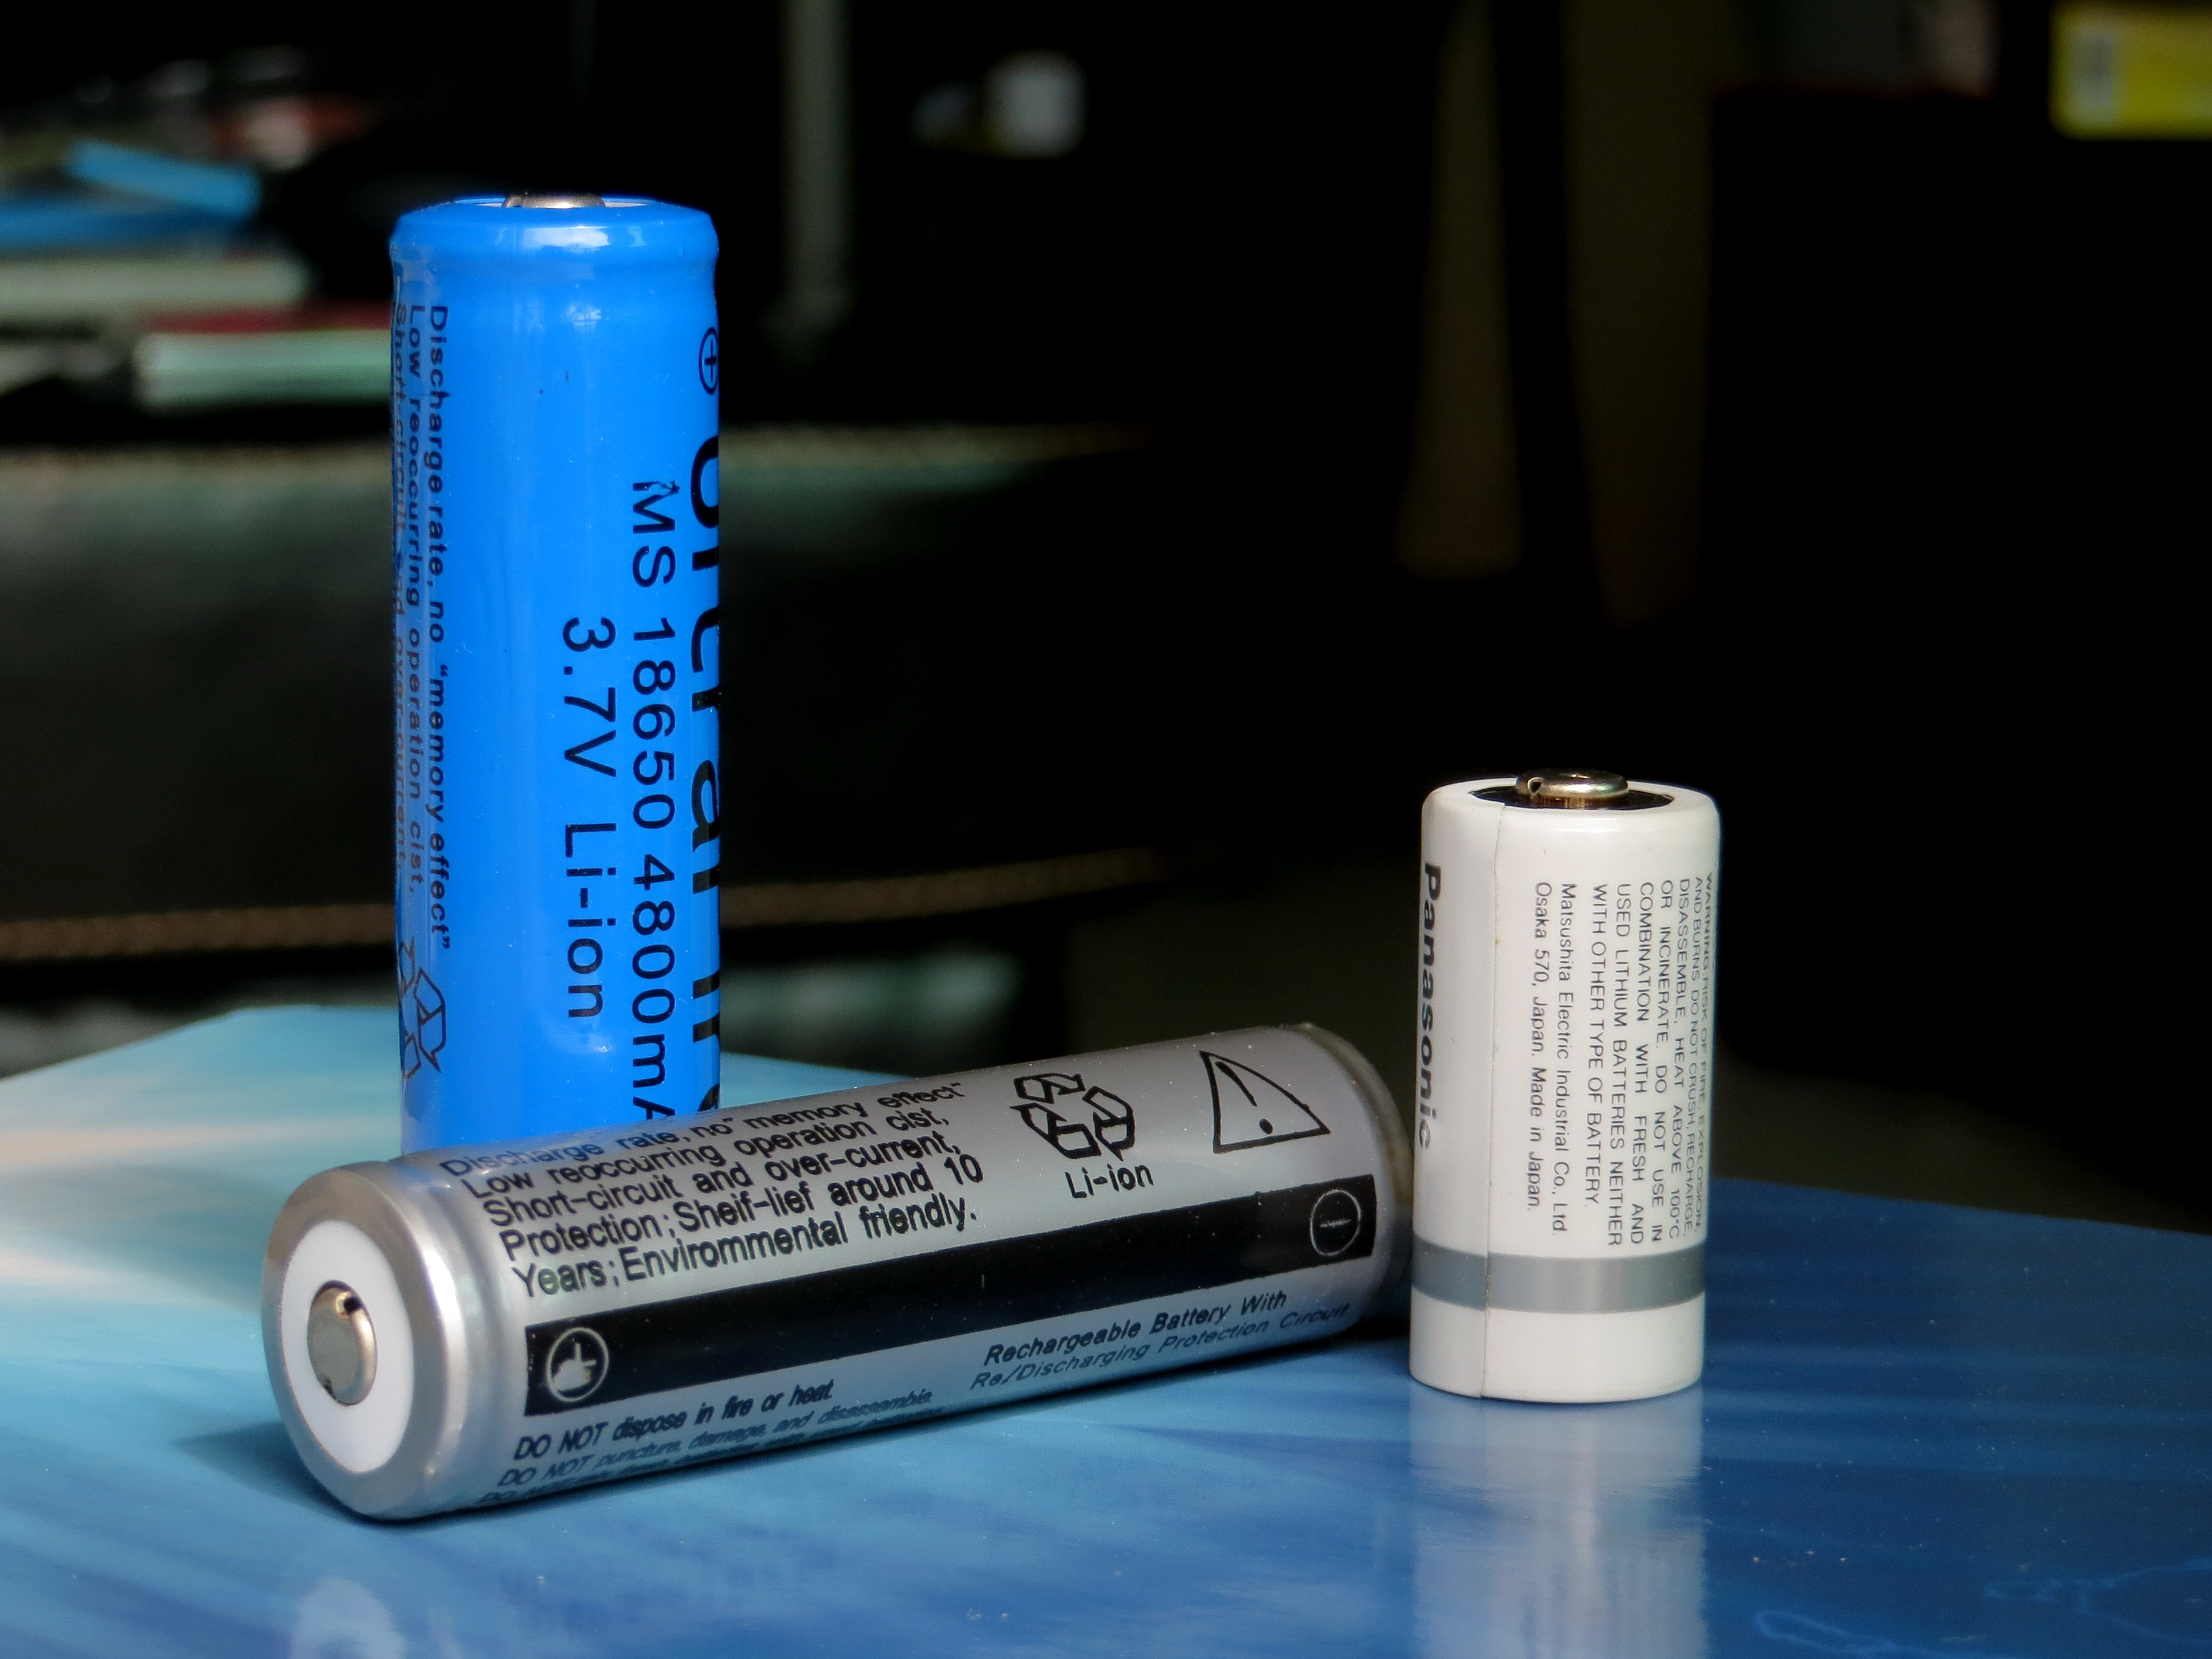
\includegraphics[scale=0.1]{imagenes/Li-ion.jpg}
   \caption{Baterías Li-ion \cite{mk2010_english_2012} }
   \label{fig:liion}
\end{figure}


\subsection{Algoritmos de carga para baterías Li-ion}
\label{sec:alg_lion}
Para la carga de las baterías Li-ion, el método más conocido es el de corriente constante-voltaje constante (CC/VC), esto 
debido a la simplicidad y fácil implementación. Durante la primera etapa de este algoritmo, se aplica una corriente constante
a la batería, hasta que el voltaje de esta alcance un valor preestablecido ($V_{preset}$), usualmente 4.2 voltios, luego se aplica 
un voltaje constante $V_{preset}$ a la batería de forma que la corriente aplicada va reduciendo su valor hasta alcanzar un valor
preestablecido, usualmente 0.1C, donde C es la capacidad de carga de la batería (en mAh), momento en el cual se considera finalizada la 
carga de la bateria \cite{shen_charging_2012}.

\begin{figure}[H]
   \centering
   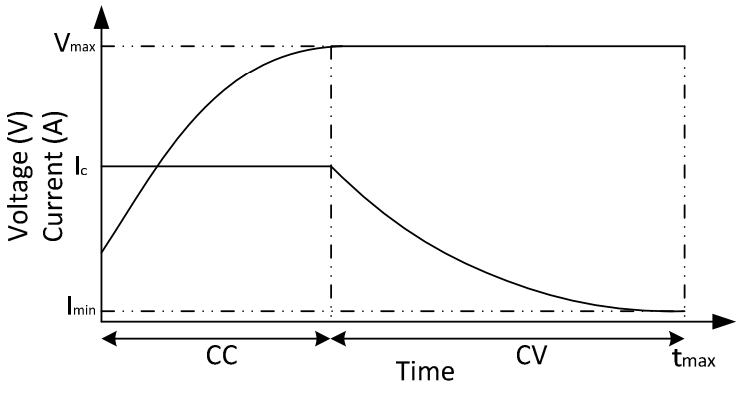
\includegraphics[scale=.6]{imagenes/perfil de carga CC-CV.png }
   \caption{Perfil de carga para el algoritmo CC/VC \cite{shen_charging_2012} }
   \label{fig:cccv}
\end{figure}


Otro algoritmo para la carga de baterías Li-Ion es el denominado \textit{Multistage current charging algorithm} (MSCC). En este
algoritmo se propone el uso de distintos valores de corriente preestablecidos  a los cuales se cargará la batería,
usualmente el cambio entre cada nivel de corriente es establecido cuando el voltaje de carga alcanza un valor determinado
(usualmente 4.2V) \cite{shen_charging_2012}. 


\begin{figure}[H]
   \centering
   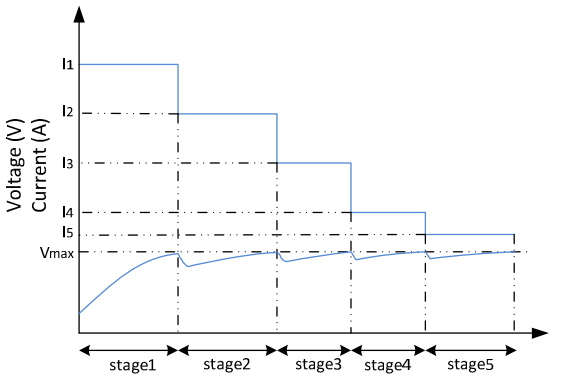
\includegraphics[scale=.75]{imagenes/perfil de carga multietapa.png}
   \caption{Perfil de carga para el algoritmo MSCC \cite{shen_charging_2012}}
   \label{fig:MSCC}
\end{figure}


\section{Baterías de Níquel metalhidruro (NiMH)}

La química de las baterías NiMH cuentan con una tecnología consolidada y ampliamente adoptada. Este tipo de baterías
tienen un menor costo comparado con las baterías basadas en litio. Los métodos de carga para este tipo de baterías son
flexibles ofreciendo corrientes de carga superiores a 1C, o una carga con corrientes bajas, lo cual reduce la demanda
de potencia hacia el sistema de alimentación, y simplificando el circuito de carga. Este tipo de baterías ofrecen altas
corrientes de descarga debido a su baja impedancia interna. Una desventaja de estas baterías es su voltaje nominal 
el cual es de 1.2V, por lo que en aplicaciones típicas es requerido el uso de 3 o 4 celdas en serie
 \cite{texas_instrumens_multi-chemistry_2022}. La densidad energética de este tipo de baterías se encuentra en el 
 rango de 40-60 Wh/Kg \cite{zhan_characteristics_1999}. En la figura \ref{fig:NiMH} se muestran dos baterías NiMH
 en formato AA.

\begin{figure} [H]
   \centering
   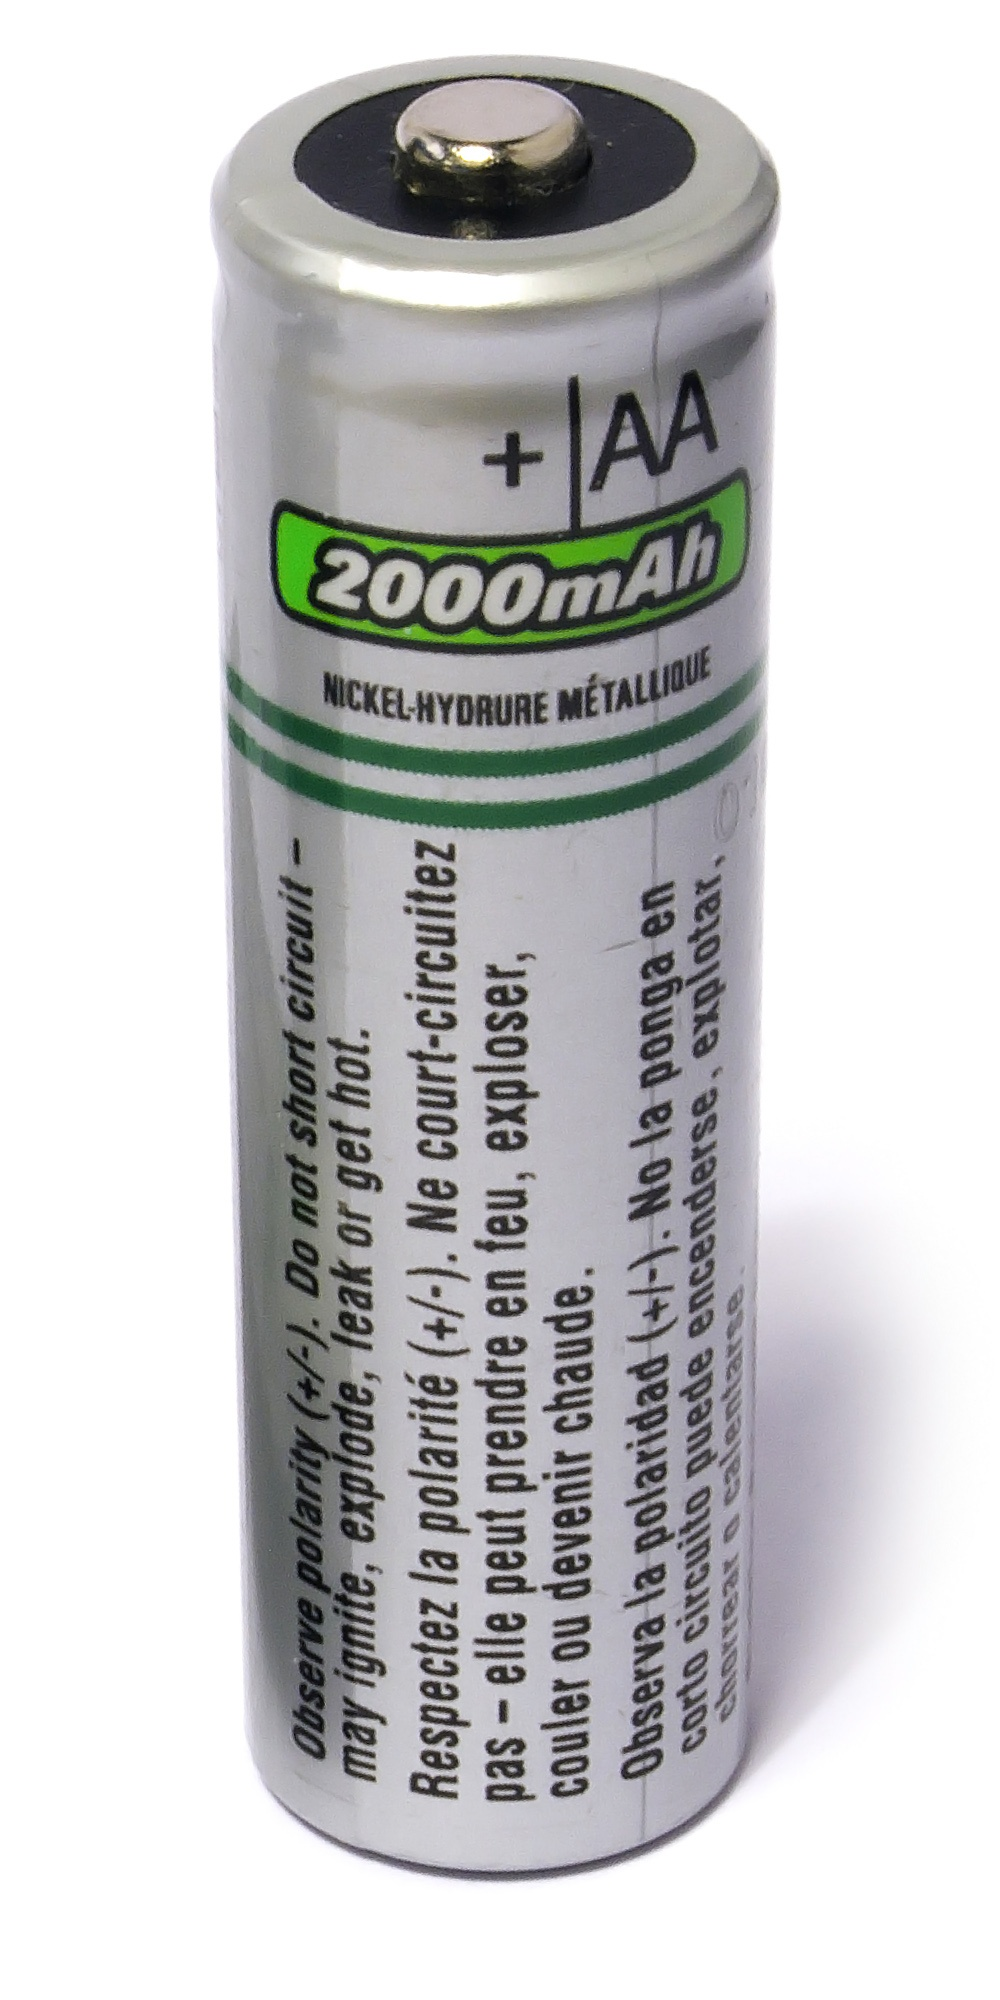
\includegraphics[scale=.1]{imagenes/NiMH.jpg}
   \caption{Batería NiMH \cite{multicherry_english_2020}}
   \label{fig:NiMH}
\end{figure}


\subsection{Algoritmos de carga para baterías NiMH}
\label{sec:alg_nimh}
El algoritmo de cambio de voltaje negativo (\textit{negative delta voltage method}) es un método de carga empleado
en las baterías NiMH que consiste en aplicar una corriente de carga constante a la batería, mientras se monitorea 
el voltaje de la misma. Para determinar cuando la batería se encuentra totalmente cargada se usa la detección de una 
caída de voltaje en la misma. Sin embargo, este método no es el más recomendado, puesto que la reacción química que se 
presenta al momento de la carga de batería es exotérmico, por lo que al momento de presentar esta caída de voltaje se 
puede presentar un aumento excesivo en la temperatura. Otra característica que hace difícil la implementación de este 
algoritmo, es el hecho de que algunos tipos de baterías NiMH no presentan una caída significativa de voltaje al momento
de alcanzar su capacidad máxima de carga \cite{nicolai_nickel-cadmium_1995}.

Un segundo método de carga consiste en aplicar una corriente de carga constante y 
detectar el punto de inflexión (punto en el que ya no existe cambio
en el voltaje de la batería) en la curva de tensión para finalizar el proceso de carga.
Esto ayuda a prevenir un sobrecalentamiento
excesivo de la batería, lo que a su vez contribuye significativamente a prolongar su vida útil. 
Para la detección del punto de inflexión es necesaria la primera derivada del voltaje de la batería con respecto 
al tiempo, en la práctica esta es aproximada mediante la medición en tiempo real \cite{nicolai_nickel-cadmium_1995}.

\section{Convertidores conmutados}

En el campo de la electrónica de potencia, el principal elemento que es esencial es el convertidor conmutado, el cual
en general consta de un puerto de potencia de entrada, un puerto de potencia de salida, asi como una señal de control,
un modelo de convertidor conmutado se puede observar en la figura \ref{fig:switching}. La potencia de entrada es procesada
con base en la señal de control del convertidor, produciendo una potencia de salida. Un tipo de convertidor comúnmente utilizado
es el convertidor DC-DC, en el cual un voltaje constante de entrada es convertido a un voltaje constante de salida que tiene 
una magnitud menor o mayor, y en algunos casos con polaridad opuesta. Adicionalmente la entrada del convertidor puede o no estar  aislada eléctricamente de la salida. Los convertidores conmutados son
ampliamente usados debido a su alta eficiencia, puesto que, teóricamente tienen una eficiencia del 
100\% a diferencia de los reguladores lineales \cite{erickson_fundamentals_2020}.

\begin{figure}[H]
   \centering
   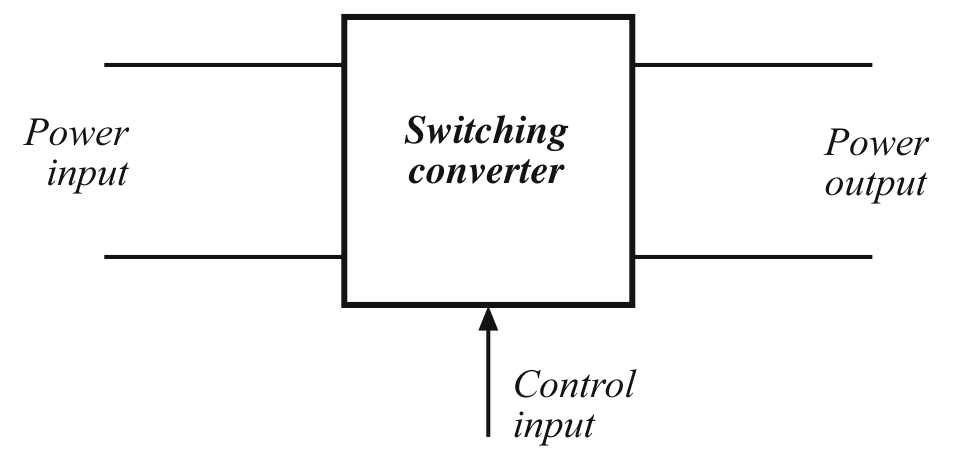
\includegraphics[scale=.4]{imagenes/switching converter.png}
   \caption{Modelo general de un convertidor conmutado \cite{erickson_fundamentals_2020}}
   \label{fig:switching}
\end{figure}

Otra parte esencial para un convertidor conmutado es el controlador,  esto ya que siempre es requerida
un voltaje de salida que se encuentre bien regulado, aun si existen variaciones en el voltaje de entrada
o en la corriente requerida por la carga \cite{erickson_fundamentals_2020}. En la figura \ref{fig:controlador} se 
presenta la topología general para un convertidor conmutado al incluir el controlador. 

\begin{figure}[H]
    \centering
    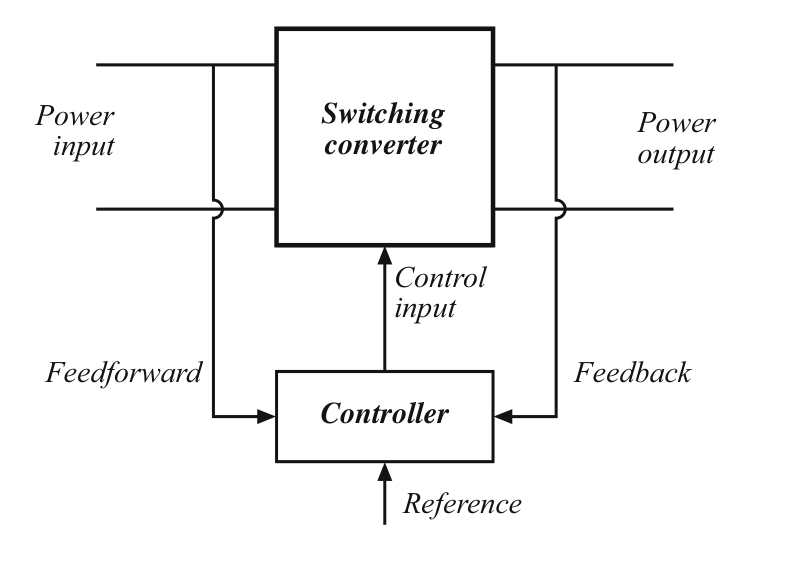
\includegraphics[scale=0.4]{imagenes/topologia.png}
    \caption{Topología general de un convertidor conmutado junto con su controlador \cite{erickson_fundamentals_2020}}
    \label{fig:controlador}
\end{figure}

Los convertidores conmutados DC-DC operan bajo dos principios el balance voltios-segundo en el inductor y el balance en la carga del capacitor, los cuales son explicados a continuación \cite{erickson_fundamentals_2020}.


\subsection{Balance voltios-segundo en el inductor}

 Este principio expresa que el cambio neto en la corriente del inductor
durante un periodo de conmutación debe ser igual a 0, debido a que en un convertidor conmutado
la corriente promedio de un inductor no debe de cambiar. Dado que la relación voltaje-corriente en un  inductor está dada por
\begin{equation}
    v_L = L \odv[order=1]{i_L}{t}
    \label{eq:VIinductor}
\end{equation}

donde $i_L$ es la corriente en el inductor, $v_L$ es el voltaje en el inductor
y $L$ la inductancia, al integrar \ref{eq:VIinductor} durante un periodo de conmutación
se tiene 
\begin{equation}
i_L\left(T_s\right)-i_L(0)=\frac{1}{L} \int_0^{T_s} v_L(t) d t
\label{eq:integralInductor}
\end{equation}

donde $T_s$ es el periodo de conmutación. En la ecuación \ref{eq:integralInductor}, el lado
derecho de la igualdad representa el cambio neto durante un periodo de conmutación, el cual 
debe ser igual a 0, teniendo como resultado

\begin{equation}
    \int_0^{T_s} v_L(t) d t = 0
\end{equation}

este resultado es importante para el análisis de convertidores DC-DC conmutados \cite{erickson_fundamentals_2020}.

\subsection{Balance en la carga del capacitor}

Este principio expresa que el cambio neto de la corriente en el capacitor durante un periodo 
de conmutación es igual a 0. Por argumentos similares a los dados en la sección anterior se 
llega a la ecuación mostrada en \ref{eq:balanceCarga} \cite{erickson_fundamentals_2020}.

\begin{equation}
    \int_0^{T_s} i_C(t) d t = 0
    \label{eq:balanceCarga}
\end{equation}

\subsection{Convertidor reductor (\textit{buck converter})}

El convertidor reductor, como su nombre lo indica, lleva a cabo la función de disminuir
 el voltaje de entrada ($V_g$, en la figura \ref{fig:buck}). Mediante el uso del principio del
balance voltios-segundo en el inductor, el balance en la carga del capacitor, y
 adicionalmente empleando la aproximación de rizado pequeño (aproximación en la cual todos los 
voltajes y corrientes en los elementos de un circuito se consideran constantes  \cite{erickson_fundamentals_2020}),
 se obtiene que la relación entre el voltaje de entrada y el de salida está dado por 
 \begin{equation}
    V=DV_g  
    \label{eq:salida_buck}
 \end{equation}
donde $D$ es el ciclo de trabajo, que es la fracción de tiempo en la que el
interruptor se encuentra en la posición 1 (ver figura \ref{fig:buck}) con
respecto al periodo de conmutación, mientras que $V$ es el voltaje 
a la salida del convertidor ($v(t)$, en la figura \ref{fig:buck})
 \cite{erickson_fundamentals_2020}. 



\begin{figure}[H]
    \centering
    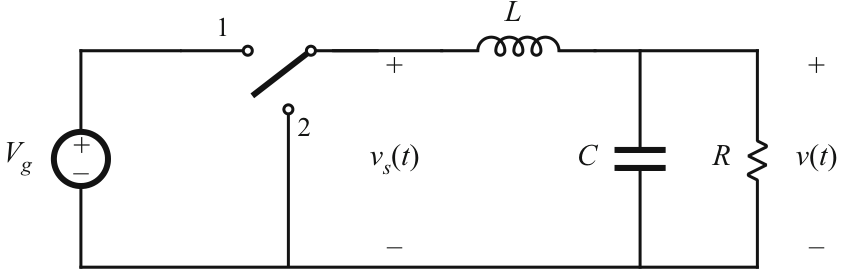
\includegraphics[scale=0.5]{imagenes/buckIdeal.png}
    \caption{Convertidor reductor con elementos ideales \cite{erickson_fundamentals_2020}}
    \label{fig:buck}
\end{figure}

Debido a que para la deducción de la relación entre voltaje de salida y 
entrada del convertidor (ecuación \ref{eq:salida_buck}) fue empleada la
aproximación de rizado pequeño, no se refleja el ruido de conmutación 
a la salida del circuito. En \cite{erickson_fundamentals_2020} se 
realiza el análisis para determinar las amplitudes, para el rizado tanto de 
la corriente del inductor como del voltaje en el capacitor (ecuaciones 
\ref{eq:ripple_L} y \ref{eq:ripple_C} respectivamente)
\begin{equation}
    \Delta I = \frac{V_g-V}{2L}DT_s
    \label{eq:ripple_L}
\end{equation}

\begin{equation}
    \Delta C = \frac{\Delta I T_s}{8C}
    \label{eq:ripple_C}
\end{equation}

En las figuras \ref{fig:ripple_L} y \ref{fig:ripple_C} se puede observar la forma de onda del voltaje
en el capacitor y la corriente en el inductor del convertidor reductor.

\begin{figure}[H]
    \centering
    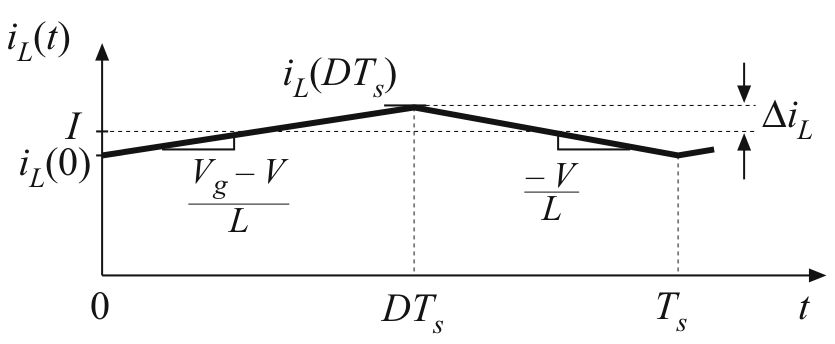
\includegraphics[scale=.5]{imagenes/buck_ripple_L.png}
    \caption{Forma de onda de la corriente en el inductor \cite{erickson_fundamentals_2020}}
    \label{fig:ripple_L}
\end{figure}

\begin{figure} [H]
    \centering
    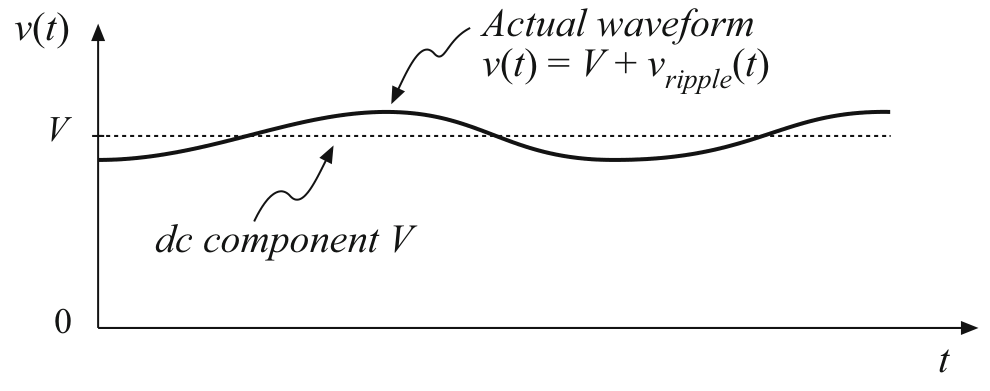
\includegraphics[scale=.4]{imagenes/buck_ripple.png}
    \caption{Forma de onda del voltaje en el capacitor \cite{erickson_fundamentals_2020}}
    \label{fig:ripple_C}
\end{figure}

\subsubsection{LM2596}

 El LM2596 es un IC el cual permite el diseño de un convertidor reductor que opera a una 
 frecuencia de $150\text{KHz}$ con conmutador integrado
por lo que únicamente es necesario añadir un inductor, diodo y capacitor de 
 forma externa para tener un convertidor reductor. 
 
 Este viene en versiones con voltajes de 
 salida fijos y también con una versión ajustable.  Para la versión ajustable la tensión de
 referencia es de 1.23 V de forma típica, este voltaje de referencia es el que busca igualar
 el controlador interno en el pin denominado \textit{feedback}. Para establecer el voltaje
 a la salida es necesario añadir 2 resistencias funcionando como divisor de voltaje, 
 de forma que se le permita al IC sensar el voltaje de salida. Para la determinación de los
valores de resistencias es utilizada la ecuación \ref{eq:lm2596}. 

 \begin{figure}[H]
    \centering
    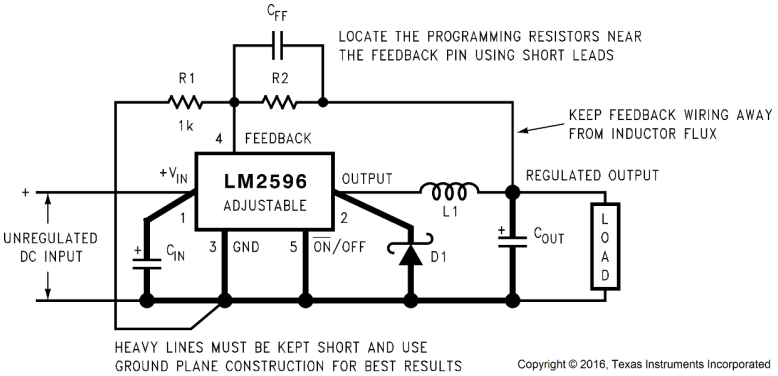
\includegraphics[scale=0.7]{imagenes/LM2596_adj.png}
    \caption{Convertidor reductor utilizando el LM2596 en su versión ajustable \cite{lm2596}}
    \label{fig:lm2596}
 \end{figure}
 
\begin{equation}
    R_2 = R_1(\frac{V_{out}}{V_{ref}} - 1)
    \label{eq:lm2596}
\end{equation}

En donde $R_1$ y $R_2$ son los las resistencias con los mismos nombres mostrados en la
figura \ref{fig:lm2596} mientras que $V_{ref}$ es el voltaje de referencia interno del
IC, y $V_{out}$ es el voltaje de salida deseado. Es posible desactivar el funcionamiento
del LM2596 aplicando un voltaje superior a 2 V, en el pin 
$\overline{\text{ON}}\backslash\text{OFF}$.

\subsection{Multiplicador de voltaje (\textit{Charge pump})}
    \label{sec:charge_pump}
    Un multiplicador de voltaje es un convertidor conmutado que permite (idealmente)
    obtener un voltaje de salida que es múltiplo entero del voltaje de entrada
    (ver ecuación \ref{eq:charge_pump}).
    
    \begin{equation}
        V_{out} = n V_{in}
        \label{eq:charge_pump}
    \end{equation}
    
    Un circuito empleado comúnmente es denominado \textit{
    Dickson charge pump} el cual es mostrado en la figura \ref{fig:dickson_charge}.
    
    \begin{figure}[H]
        \centering
        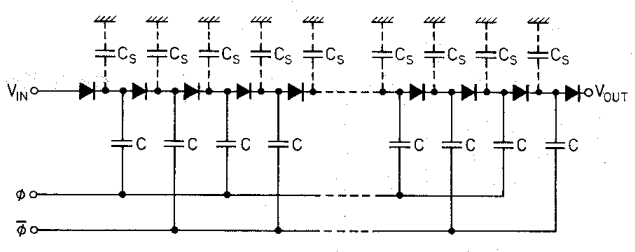
\includegraphics[scale=1]{imagenes/Positive_dickson_charge.png}
        \caption{\textit{ Dickson charge pump} \cite{charge_dikson}}
        \label{fig:dickson_charge}
    \end{figure}

    En \cite{charge_dikson} se realiza el análisis del circuito mostrado
    en la figura \ref{fig:dickson_charge}, con
    el cual se obtiene que la relación entre voltaje de entrada y salida está dada
    por la ecuación \ref{eq:dickson_charge}.

    \begin{equation}
        V_{out} = V_{in} + N \left (  \frac{C}{C+C_s}V_\Phi - V_D - 
        \frac{I_{out}}{(C+C_s)f} \right )
        \label{eq:dickson_charge}
    \end{equation}

    En donde $N$ es el número de etapas en el convertidor, $C$ es la capacitancia
    entre cada etapa y el nodo $\Phi$ o $\bar{\Phi}$, $f$ es la frecuencia de 
    operación del multiplicador de voltaje, $V{\Phi}$ es la amplitud
    de la señal en los nodos $\Phi$ y $\bar{\Phi}$, $C_s$ son capacitancias parásitas,
    $I_{out}$ es la corriente de salida del
    convertidor y $V_D$ es la caída de voltaje en el diodo.

    Este mismo convertidor puede ser empleado para obtener un voltaje de salida
    menor al de entrada (es decir voltajes negativos), para ello es necesario
    realizar un intercambio entre la carga del circuito y el voltaje de entrada,
    Por lo que en la ecuación \ref{eq:dickson_charge} $V_{in}$ y $V_{out}$
    son intercambiados \cite{mohammad_switched_2010}. En la figura 
    \ref{fig:dickson_charge_bid} se muestra el intercambio entre carga y 
    voltaje de entrada en el \textit{Dickson charge pump}.
    
    \begin{figure}[H]
        \centering
        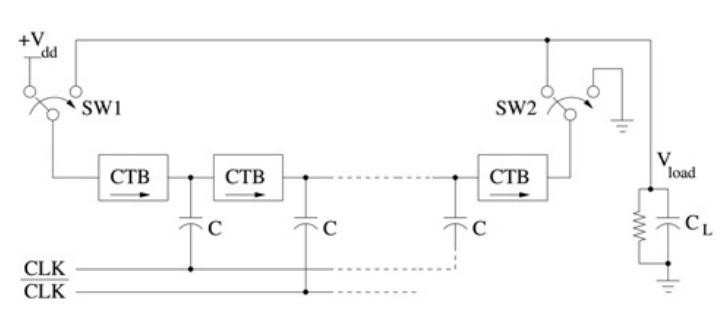
\includegraphics[scale=0.75]{imagenes/positive_negative_charge_pump.png}
        \caption{intercambio entre carga y voltaje de entrada en el
                 \textit{Dickson charge pump} (CTB, \textit{charge transfer
                 block} en la figura \ref{fig:dickson_charge} son implementados
                 con diodos) \cite{mohammad_switched_2010}}
        \label{fig:dickson_charge_bid}
    \end{figure}

    Al intercambiar el voltaje de entrada y salida de la ecuación \ref{eq:dickson_charge},
    y aplicando $0$V en la entrada (que es el caso mostrado en la figura 
    \ref{fig:dickson_charge_bid}, cuando SW1 y SW2 se encuentran cerrados 
    con el contacto de la derecha) se tiene que la relación entre voltaje de entrada
    y salida está dada por la ecuación \ref{eq:dickson_charge_neg}.

    \begin{equation}
        V_{out} = - N \left (  \frac{C}{C+C_s}V_\Phi - V_D - 
        \frac{I_{out}}{(C+C_s)f} \right )
        \label{eq:dickson_charge_neg}
    \end{equation}


\section{Multiplexores de potencia}

Un multiplexor de potencia, es un conjunto de conmutadores electrónicos que son utilizados
para seleccionar entre dos o más entradas de potencia, hacia una única salida. El uso de 
multiplexores de potencia le brinda la flexibilidad a un sistema de poder seleccionar
entre diferentes tipos de entradas de potencia \cite{triano_basics_2020}. En la figura 
\ref{fig:powerMux} se muestra el diagrama de bloques de un multiplexor de potencia.


\begin{figure}[H]
    \centering
    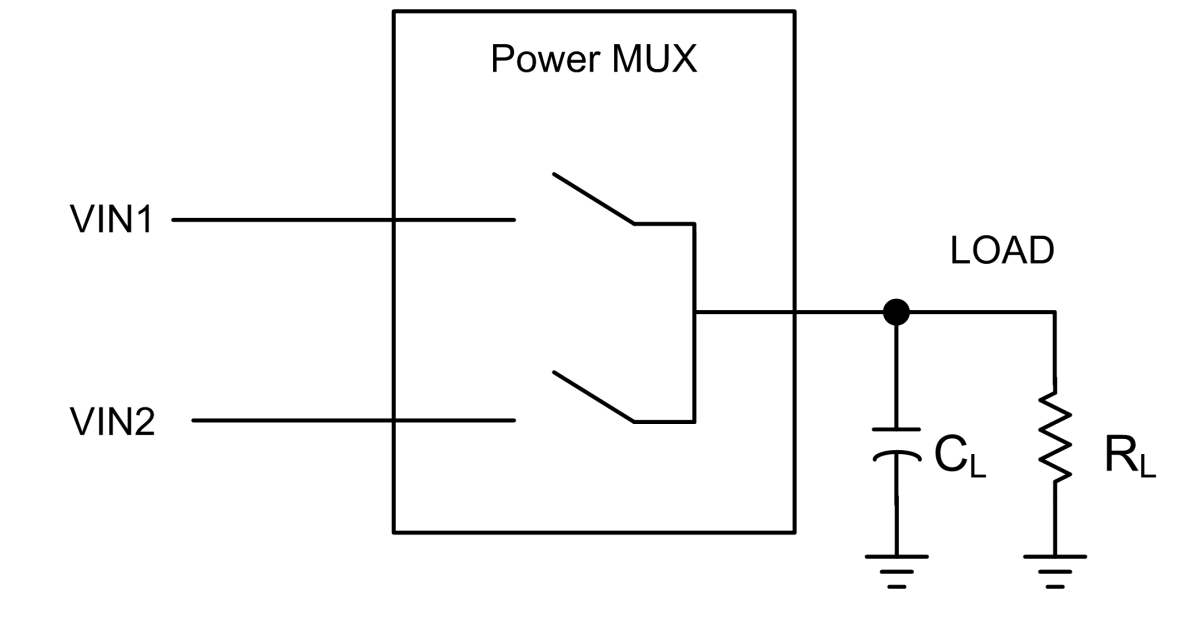
\includegraphics[scale=.35]{imagenes/powerMux.png}
    \caption{Diagrama de bloques de un multiplexor de potencia \cite{triano_basics_2020}}
    \label{fig:powerMux}
\end{figure}


En el caso de que no exista preferencia para alguna de las alimentaciones de entrada, o inclusive
si siempre se prefiere el uso del voltaje de entrada más alto, el requerimiento mínimo para un multiplexor
de potencia es el bloqueo de corriente inversa. Este requerimiento puede ser cumplido mediante el uso de 
diodos o circuitos integrados que se comporten como diodos \cite{triano_basics_2020}.  Como se muestra en la figura \ref{fig:muxDiode}.

\begin{figure}[H]
    \centering
    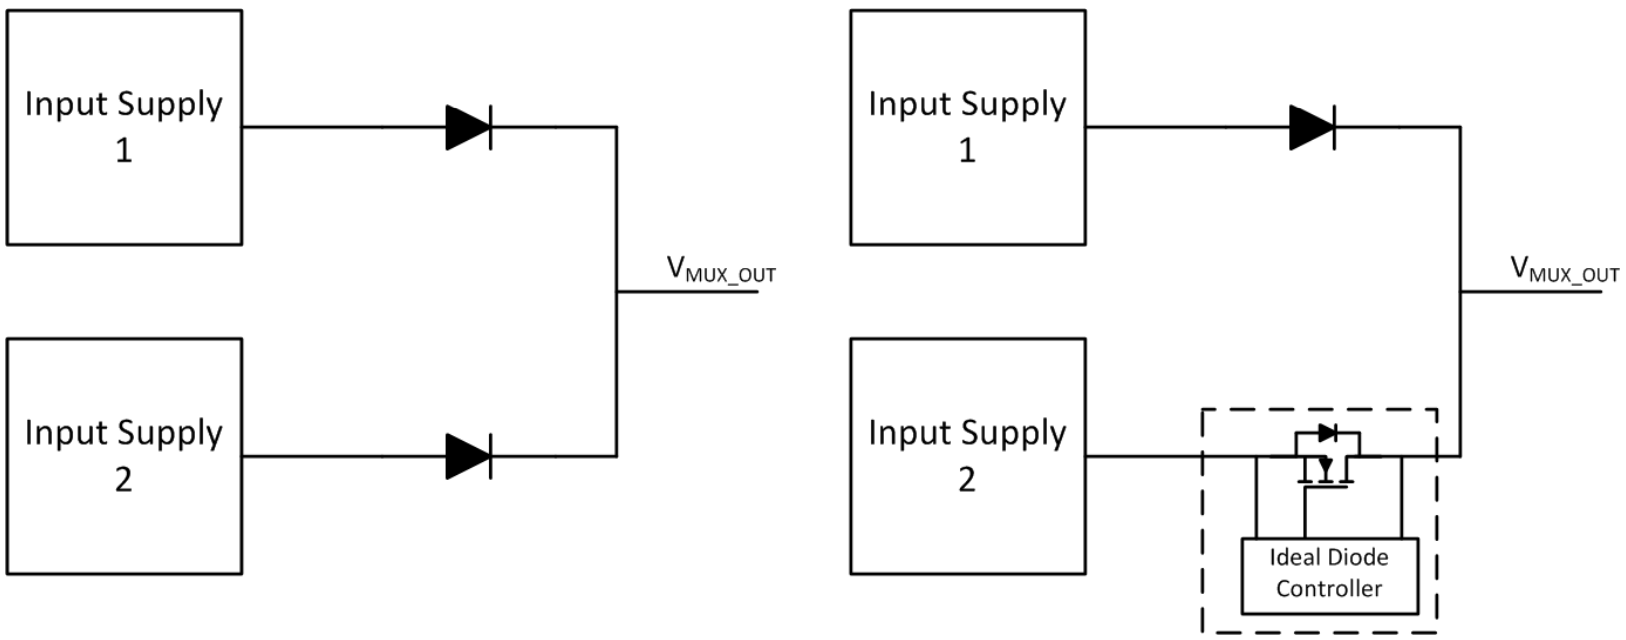
\includegraphics[scale=.3]{imagenes/minimumMux.png}
    \caption{Sistema mínimo para un multiplexor de potencia \cite{triano_basics_2020}}
    \label{fig:muxDiode}
\end{figure}

En el caso de que exista alguna prioridad para los voltajes de entrada, es necesario agregar conmutadores,
por ejemplo un transistor MOSFET, para tener un control total sobre la ruta que será habilitada. Al igual que
en el caso sin prioridad, el bloqueo ante corrientes inversas debe seguir presente \cite{triano_basics_2020}. En la figura \ref{fig:priorityMux} se muestra un ejemplo de multiplexor de potencia con prioridad.

\begin{figure}[H]
    \centering
    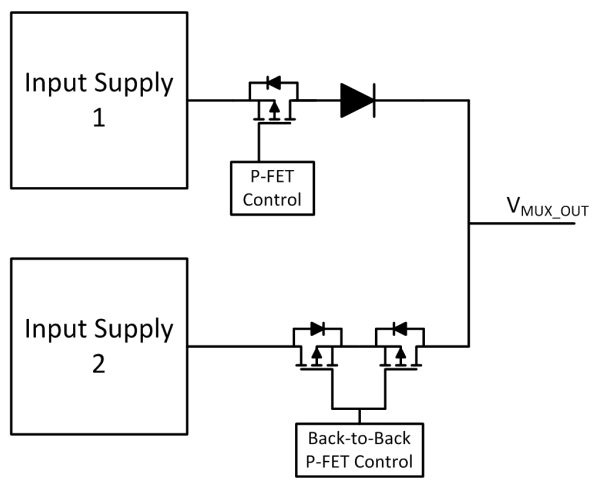
\includegraphics[scale=.5]{imagenes/priorityMUX.png}
    \caption{Multiplexor de potencia con prioridad \cite{triano_basics_2020}}
    \label{fig:priorityMux}
\end{figure}

Para el control de multiplexores de potencia, se tienen dos opciones: manual o automático. Un multiplexor de
potencia manual es aquel en el cual cada fuente de alimentación es seleccionada mediante señales externas. Por el contrario, un multiplexor automático es aquel que no requiere señales externas para el cambio entre 
una fuente de alimentación y otra, en este tipo de control usualmente existe una entrada de potencia que 
tiene la prioridad.

\section{Pololu 3Pi+}

El Pololu 3Pi+ es un robot, programable por el usuario. Este se encuentra basado en el microcontrolador ATmega32U4 AVR
de microchip, el microcontrolador incorporado se encuentra preprogramado con un gestor de arranque que es compatible
 Con la plataforma Arduino. Incluye dos puentes H para el control de los motores así como distintos sensores, como lo 
 son \textit{encoders} de cuadratura, así como una unidad de medición inercial \cite{noauthor_pololu_nodate}. En cuanto 
 al sistema de potencia tiene como principal fuente de energía el uso de cuatro celdas AAA en serie, en donde el 
 terminal negativo se encuentra conectado a GND mientras que el terminal positivo, al pin denominado VBAT (ver figura
 \ref{fig:power}).

 \begin{figure}[H]
    \centering
    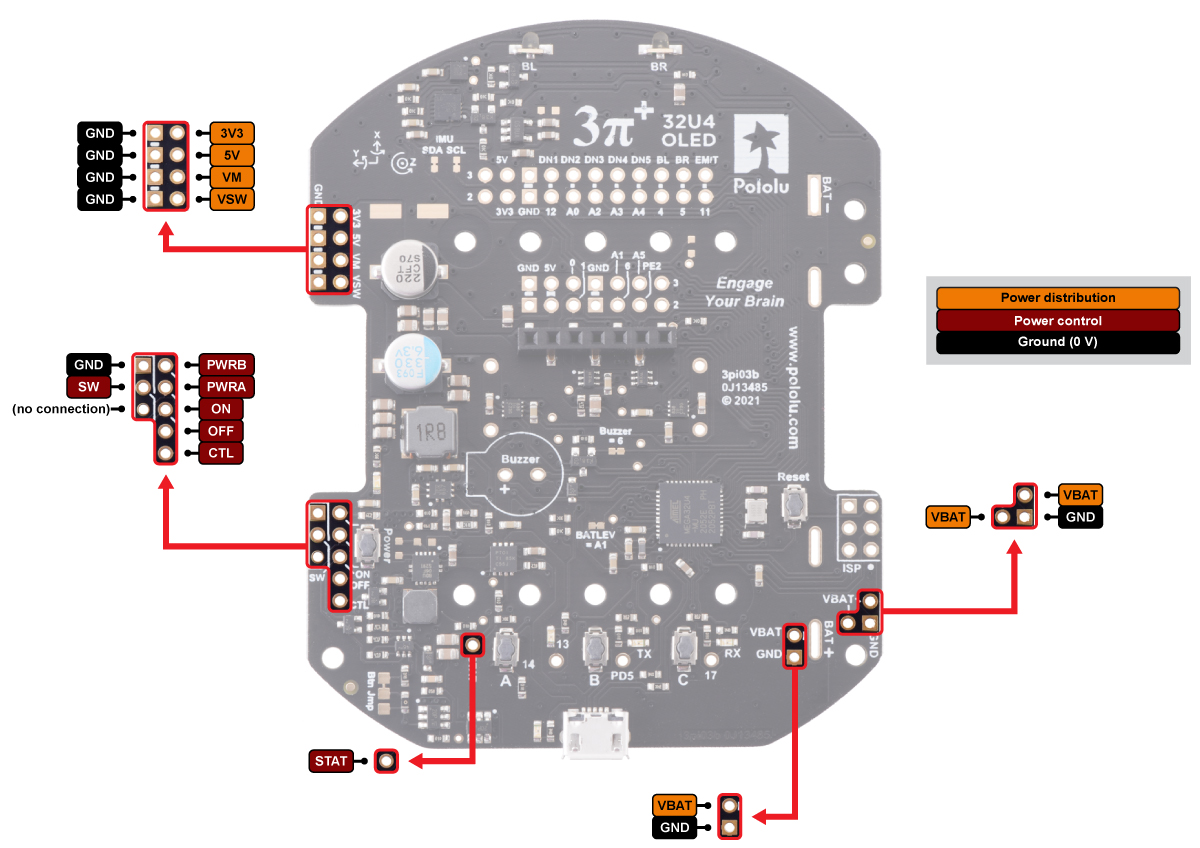
\includegraphics[scale=.2]{imagenes/PololuPower.jpg}
    \caption{Distribución de los pines de potencia el Pi3+ \cite{noauthor_pololu_nodate}}
    \label{fig:power}
 \end{figure}

 Para la alimentación de los motores, el Pi3+ posee un convertidor conmutado, para proveer de 8 voltios a los motores
 de forma que no se presente una caída en la velocidad de los motores debido a la descarga gradual de las baterías,
 adicionalmente, se tiene un segundo regular conmutado que provee 5 voltios, aunque esta no es accesible de forma directa
 para el usuario. También posee un regulador lineal (LDO por sus siglas en inglés). El voltaje de entrada (el cual es 
 utilizado para generar los 8, 5 y 3.3 voltios de la placa) es seleccionado mediante un multiplexor de potencia, más 
 específicamente se emplea el circuito integrado (IC) TPS2113A fabricado por Texas Instruments \cite{noauthor_pololu_nodate}.

\section{Amplificador operacional}

Un amplificador operacional es un amplificador con una alta ganancia,
alta impedancia de entrada y baja impedancia de salida. Posee dos entradas
las cuales son denominadas entrada inversora, entrada no inversora. La salida
del amplificador operacional es la diferencia entre las dos entradas multiplicada
por la ganancia del amplificador operacional \cite{electronic_Boylestad}. En 
la figura \ref{fig:ampOp} se muestra el símbolo de un amplificador operacional.

\begin{figure}[H]
    \centering
    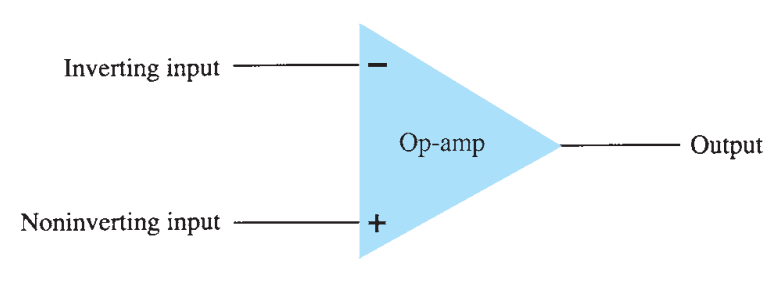
\includegraphics[scale=0.5]{imagenes/ideal_opamp.png}
    \caption{Símbolo de un amplificador operacional \cite{electronic_Boylestad}}
    \label{fig:ampOp}
\end{figure}

La ecuación que describe el comportamiento de un amplificador operacional es la siguiente
\begin{equation}
    V_{out} = A(V^+ - V^-)
    \label{eq:ampOp}
\end{equation}

Una consecuencia de que la ganancia del amplificador operacional sea muy alta, es que
la diferencia entre las entradas inversora y no inversora es muy pequeña, por lo que
se puede considerar que ambas entradas tienen el mismo voltaje. Esta característica
es conocida como "cortocircuito virtual" \cite{electronic_Boylestad}.

 El hecho de tener una 
impedancia de entrada infinita implica que no existe corriente de entrada, por lo que
la corriente que entra por la entrada inversora y no inversora es igual a 0. 

\subsection{Amplificador diferencial}
\label{sec:ampDif}
Un amplificador diferencial es un amplificador operacional que tiene dos entradas
y una salida. La salida de este amplificador es la diferencia entre las dos entradas
multiplicada por la ganancia del amplificador diferencial. En la figura \ref{fig:ampDif}
se muestra el diagrama de un amplificador diferencial \cite{electronic_Boylestad}.

\begin{figure}[H]
    \centering
    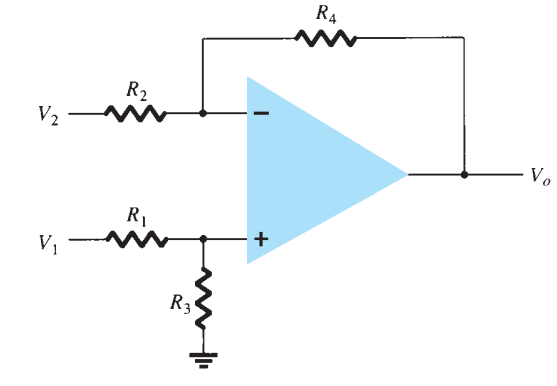
\includegraphics[scale=0.5]{imagenes/ampDif.png}
    \caption{Diagrama de un amplificador diferencial \cite{electronic_Boylestad}}
    \label{fig:ampDif}
\end{figure}

La ecuación que describe el comportamiento de un amplificador diferencial es la siguiente:
\begin{equation}
    V_{out} =  \frac{R_3(R_2+R_4)}{R_2(R_1+R_3)}V_2 - \frac{R_4}{R_2}V_1
    \label{eq:ampDif}
\end{equation}

Si el valor de $R_1$ es igual a $R_2$ y el valor de $R_3$ es igual a $R_4$, la ecuación
\ref{eq:ampDif} se puede simplificar a la ecuación \ref{eq:ampDifSimp}.

\begin{equation}
    V_{out} =  \frac{R_4}{R_2}(V_2 - V_1)
    \label{eq:ampDifSimp}
\end{equation}
	\fi
\fi

% CAPÍTULOS
% ------------------------------------------------------------------------------
\newpage
\ifdefined\parpordefecto
	\defaultparformat{j-capitulos}
\else
	\chapter{Sistema de carga multiquímica}

Para la carga de la batería Li-ion se escogió el método de carga CC/VC
descrito en la sección \ref{sec:alg_lion}, la máxima corriente de carga
se estableció en $1\text{A}$. Para la carga de la batería NiMH se utilizó
el método de carga de cambio de voltaje negativo descrito en la sección 
\ref{sec:alg_nimh}. Se empleó el mismo convertidor reductor para la carga
de ambas baterías, por lo que no es posible cargar ambas al mismo tiempo.
Para determinar que batería será cargada se utilizó un multiplexor de potencia
construido con transistores MOSFET de canal P.


    \section{Convertidor reductor}

    \label{sec:buck_design}

    El sistema de carga multiquímica debe ser capaz de  proporcionar una 
    corriente constante para la carga de ambos tipos de baterías. Para ello
    se decidió emplear un convertidor reductor, el cual tiene por componente principal
    el circuito integrado LM2596. Para poder realizar un control del voltaje de salida ( y de
    forma indirecta la corriente del mismo)
    de forma electrónica, es decir aplicando un voltaje, se realizó una modificación al circuito
    de realimentación del circuito como es mostrado en la figura \ref{fig:buck_modificado}.

    \begin{figure}[H]
        \centering
        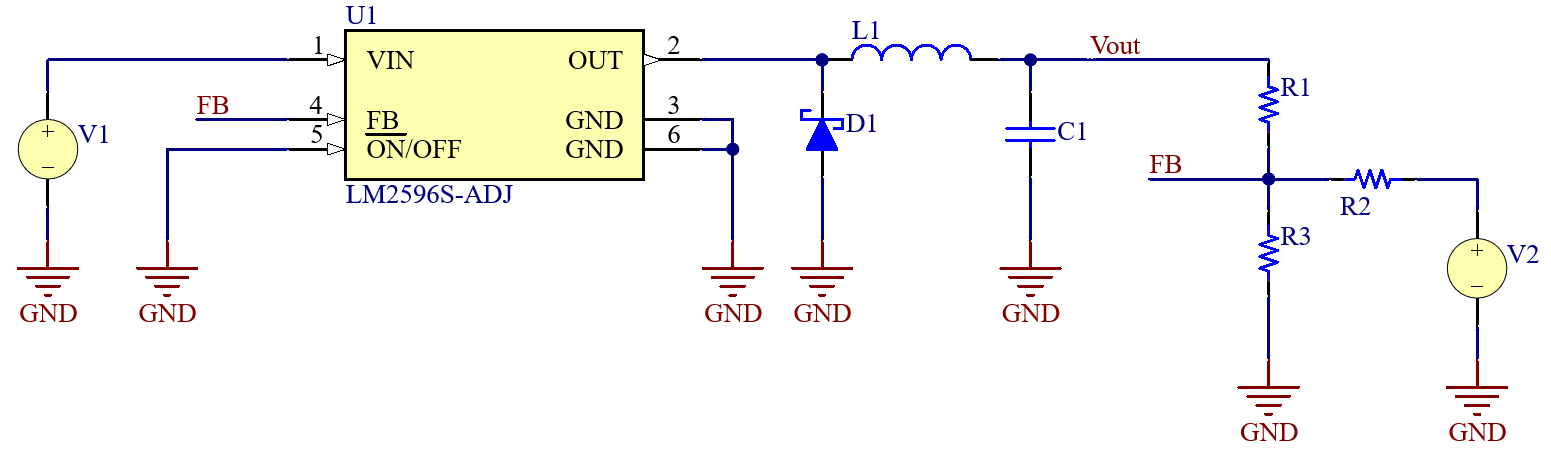
\includegraphics[scale=0.35]{imagenes/buck_control_simplificado.png}
        \caption{Convertidor reductor con realimentación modificación (versión simplificada) }
        \label{fig:buck_modificado}
    \end{figure}

    Para este convertidor se definieron los siguientes parámetros de rendimiento:

    $$ \Delta I = 150 \text{mA} $$
    $$ \Delta V = 1 \text{mV}$$

    Otros parámetros útiles para el diseño de este convertidor serán el voltaje
    de alimentación ($V_g$), así como la frecuencia de conmutación, $f_s$ (dada por la hoja 
    de datos del fabricante), los valores son:

    $$V_g = 12\text{V}$$
    $$ f_s = \frac{1}{T_s} = 150 \text{KHz}$$



    \subsection{Cálculo de resistencias para el circuito de retroalimentación}

    \label{sec:res_ret}

    Para poder determinar en que forma va a variar el voltaje en el nodo $V_{out}$ se realizó un 
    análisis de nodos en el nodo FB correspondiente a la figura \ref*{fig:buck_modificado}, 
    obteniendo la ecuación \ref*{eq:buck_control}.

    \begin{equation}
        V_{FB} = \frac{R_1R_2}{R_1R_2+R_3(R_1+R_2)} V_{out} + \frac{R_1R_3}{R_1R_3+R_2(R_1+R_3)} V_2
        \label{eq:buck_control}
    \end{equation}

    Donde $V_2$ el voltaje aplicado de forma externa para modificar el valor
    de voltaje a la salida. De la ecuación \ref*{eq:buck_control} se puede 
    observar que el valor de $V_{FB}$ es dependiente tanto de $V_2$ como de
    $V_{out}$. 

    Para determinar los valores de las resistencias se armó un sistema de dos ecuaciones,
    fijando los valores de $V_{FB}$,$V_{out}$,$V_2$, y $R_1$. Los dos valores necesarios
    de $V{out}$ se obtuvieron fijando el valor mínimo y máximo que podría tener a la salida
    el convertidor, los cuales fueron de $2.8\text{V}$ y $6.4\text{V}$ de forma que pueda usarse tanto para 
    cargar la celda de batería Li-ion, así como las 4 celdas NiMH. El valor de $V_{FB}$ 
    es el voltaje de referencia del IC LM2596. Los valores del voltaje de control se
    establecieron de forma que, cuando $V_2 = 5\text{V}$ el voltaje a la salida sea de 
    $2.8\text{V}$ mientras que cuando  $V_2 = 0\text{V}$ el voltaje sea de $6.4\text{V}$.
    Por último, se escogió un valor de $750\Omega$ para $R_1$ de forma arbitraria, siguiendo
    la recomendación de la hoja de datos del LM2596.

    Con lo explicado anteriormente, el sistema de ecuaciones a resolver es el siguiente:
    \begin{eqnarray}
        \frac{750R_3}{ 750R_3 + R_2(750 + R_3)} 6.4\text{V} = 1.23\text{V} \\
        \frac{750R_3}{ 750R_3 + R_2(750 + R_3)} 2.8\text{V} + \frac{750R_2}{750R_2+R_3(750+R_2)} 5\text{V} = 1.23\text{V}   
    \end{eqnarray}
    dando como resultado los siguientes valores para $R_2$ y $R_3$:

    $$R_2 = 2596.64\Omega$$ 
    $$R_3 = 3606.44\Omega$$

    Puesto que estos valores no son comerciales, se emplearon valores de resistencias en 
    paralelo, de forma que sea posible aproximar estos valores. Para el valor de $R_2$ 
    se empleó una resistencia de $3\text{K}\Omega$ y $20\text{K}\Omega$ dando como 
    resistencia equivalente $2.608\text{K}\Omega$. De igual forma se utilizó una 
    resistencia de $4.7\text{K}\Omega$ en paralelo con una de $15\text{K}\Omega$ para aproximar
    el valor de $R_3$, dando una resistencia total de $3.578\text{K}\Omega$.

    Al reemplazar en la ecuación \ref{eq:buck_control} los valores para $R_2$ y $R_3$ utilizados, 
    y dando un valor a $V_2$ de $5\text{V}$ se obtiene que el valor de $V_{out}$ es de $2.786\text{V}$
    mientras que si se reemplaza con $V_2 = 0\text{V}$ se obtiene que el valor de $V_{out}$ es de
    $6.431\text{V}$, los cuales son valores aceptables para la carga de ambas baterías,
    de forma que la variación en las resistencias no afecta significativamente
    el rango de operación del convertidor.

    \subsection{Componentes externos del convertidor}

        Los componentes externos necesarios para que el convertidor esté completo, son el 
        diodo $D_1$, el inductor $L_1$, y el capacitor $C_1$ que se muestran en la figura
        \ref{fig:buck_modificado}.

        Para $D_1$ se escogió el diodo 1N5817, el cual es un diodo \textit{
        schotky}, la elección de este componente fue debido a su baja caída de voltaje
        ($0.45\text{V}$ al conducir $1\text{A}$) lo cual minimiza las pérdidas por 
        conducción del mismo, mejorando la eficiencia del convertidor.

        Ya que el valor del inductor es dependiente
        del valor del voltaje a la salida del convertidor es necesario determinar cuál
        sería el valor óptimo. Para ello se definió la función $L(V)$ a partir de las 
        ecuaciones \ref{eq:ripple_L} y \ref{eq:salida_buck}. La función es la siguiente: 

        \begin{equation}
            L(V) = \frac{V_g - V}{2\Delta I}\frac{V}{V_g} T_s
            \label{eq:L_function}
        \end{equation}

        Posteriormente se obtuvo que el valor en
        donde la de derivada de $L(V)$ tiene un valor de cero es en $V = \frac{V_g}{2}$,
        por lo tanto, el valor máximo que tomará $L(V)$ será de 

        $$ L =  \frac{T_sV_g}{8\Delta I}$$
        
        Reemplazando los valores en la ecuación anterior se obtiene que el valor de 
        $L_1$ para el cual se asegura como máximo un rizado de $150 \text{mA}$ en 
        todo el rango de operación, es de $66.6 \mu \text{H}$, por lo que se usó un
        inductor de $68 \mu \text{H}$. Este aumento en el valor del inductor no afecta
        de manera negativa el funcionamiento del convertidor, ya que el valor calculado
        anteriormente unicamente es un límite inferior para el valor del inductor, un 
        valor mas alto reducirá a un mas el rizado en la corriente de salida, lo que 
        mejora el funcionamiento del convertidor.

        Por último, se empleó la ecuación \ref{eq:ripple_C} para obtener el valor 
        de $C_1$, siendo este de $125 \mu\text{F}$, por lo que se utilizó un capacitor
        electrolítico de $220 \mu\text{F}$ debido a que es el siguiente valor comercial 
        más alto disponible. De igual forma que con el inductor, el
        aumento en el valor del capacitor no afecta de manera negativa el funcionamiento
        del convertidor, ya que el valor calculado anteriormente es un límite inferior
        para el valor del capacitor, un valor más alto reducirá a un más el rizado en
        el voltaje de salida.

    \subsection{Componentes adicionales}

        Para asegurar un funcionamiento óptimo en \cite{lm2596}, se aconseja incorporar
        un capacitor en paralelo con la resistencia $R_2$ mostrada en la figura
        \ref{fig:buck_modificado}. La elección del valor de este condensador se basó
        en las pautas proporcionadas en el cuadro \ref{tb:feedforward_cap}. 
        Dado que el voltaje de salida mínimo es de $2.8\text{V}$, se optó por utilizar
        un capacitor de $33\text{nF}$.

        \begin{table}[H]
            \centering
            \begin{tabular}{|c|c|}
                \hline
                Voltaje de salida (V) & Capacitor \\
                \hline
                2 & $33\text{nF}$ \\
                4 & $10\text{nF}$ \\
                6 & $3.3\text{nF}$ \\
                9 & $1.5\text{nF}$ \\
                12 & $1\text{nF}$ \\
                15 & $680\text{pF}$ \\
                24 & $220\text{pF}$ \\
                28 & $220\text{pF}$ \\
                \hline
            \end{tabular}
            \caption{Valores para capacitancia de retroalimentación según \cite{lm2596}
                con respecto al voltaje de salida.}
            \label{tb:feedforward_cap}
        \end{table}



        Otro componente adicional necesario es un capacitor de desacople a la entrada
        del LM2596 para mejorar la estabilidad del voltaje de alimentación. Para su
        selección se empleó como criterio el uso de la figura \ref{fig:rms_cap}. Según
        \cite{lm2596} es necesario asegurar que el capacitor de salida pueda tolerar
        una corriente RMS entre el $50\%$ y $75\%$ de la corriente de salida.
        Para dar un mayor margen, se decidió escoger un capacitor que soporte una corriente
        RMS igual a la corriente máxima esperada, por lo que se escogió un capacitor
        de $470\mu\text{F}$ a $25\text{V}$.

        \begin{figure}[H]
            \centering

            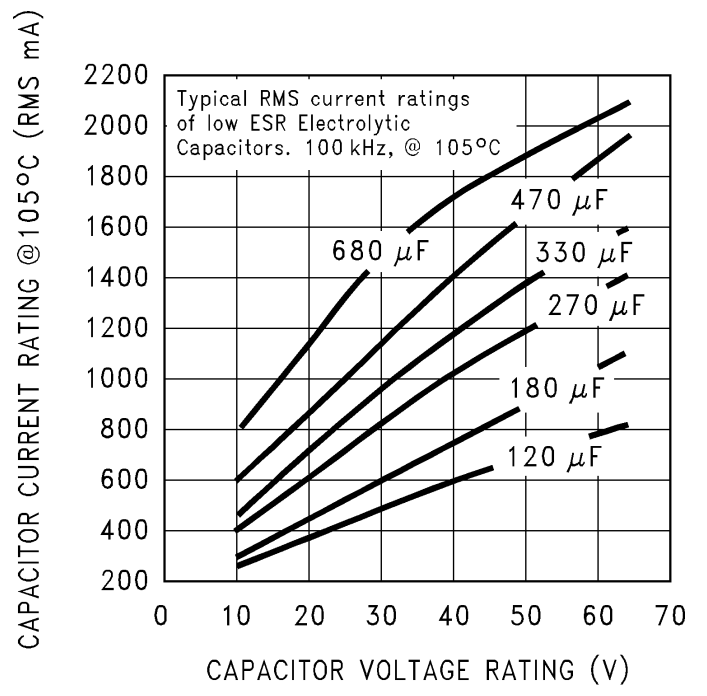
\includegraphics[scale=.4]{imagenes/rms_cap.png}
            \caption{capacidad de corriente RMS}
            \label{fig:rms_cap}

        \end{figure}

        Con todo lo discutido anteriormente, el diseño del convertidor reductor es mostrado
        en la figura \ref{fig:buck_finalizado}.

\begin{figure}[H]
    \centering

    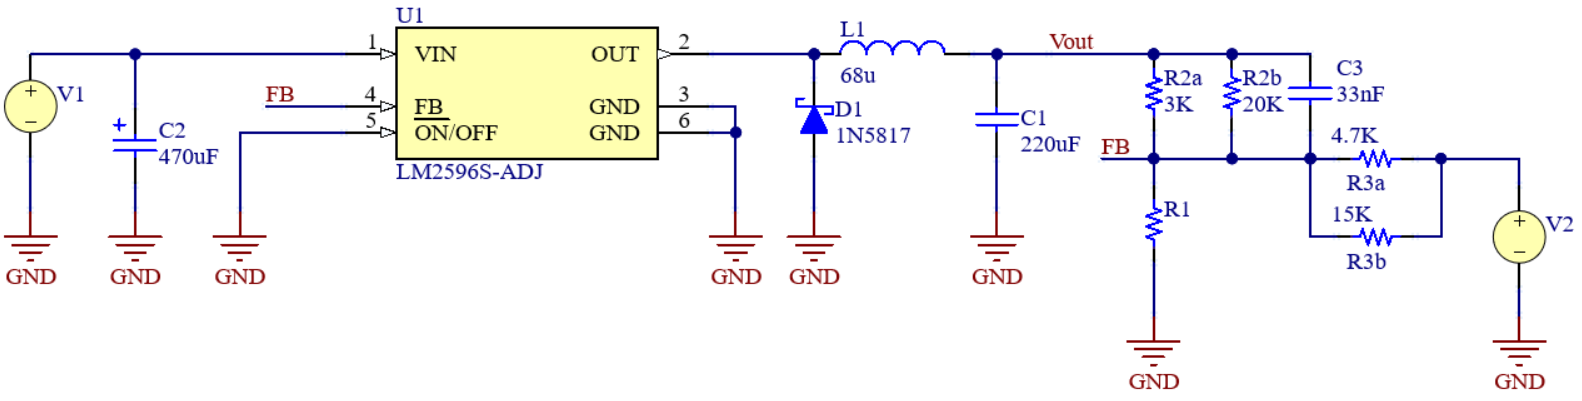
\includegraphics[scale=.45]{imagenes/buck_control_finalizado.png}
    \caption{Diseño del convertidor reductor finalizado}
    \label{fig:buck_finalizado}
\end{figure}

\subsection{Simulación del convertidor diseñado}

Para comprobar el correcto funcionamiento se realizó una simulación del 
convertidor diseñado. Para ello se empleó el simulador LTspice, junto con 
el modelo spice proporcionado por texas instruments para el circuito integrado
LM2596 (descarga disponible en \cite{noauthor_lm2596_nodate}). 

\begin{figure}[H]
    \centering
    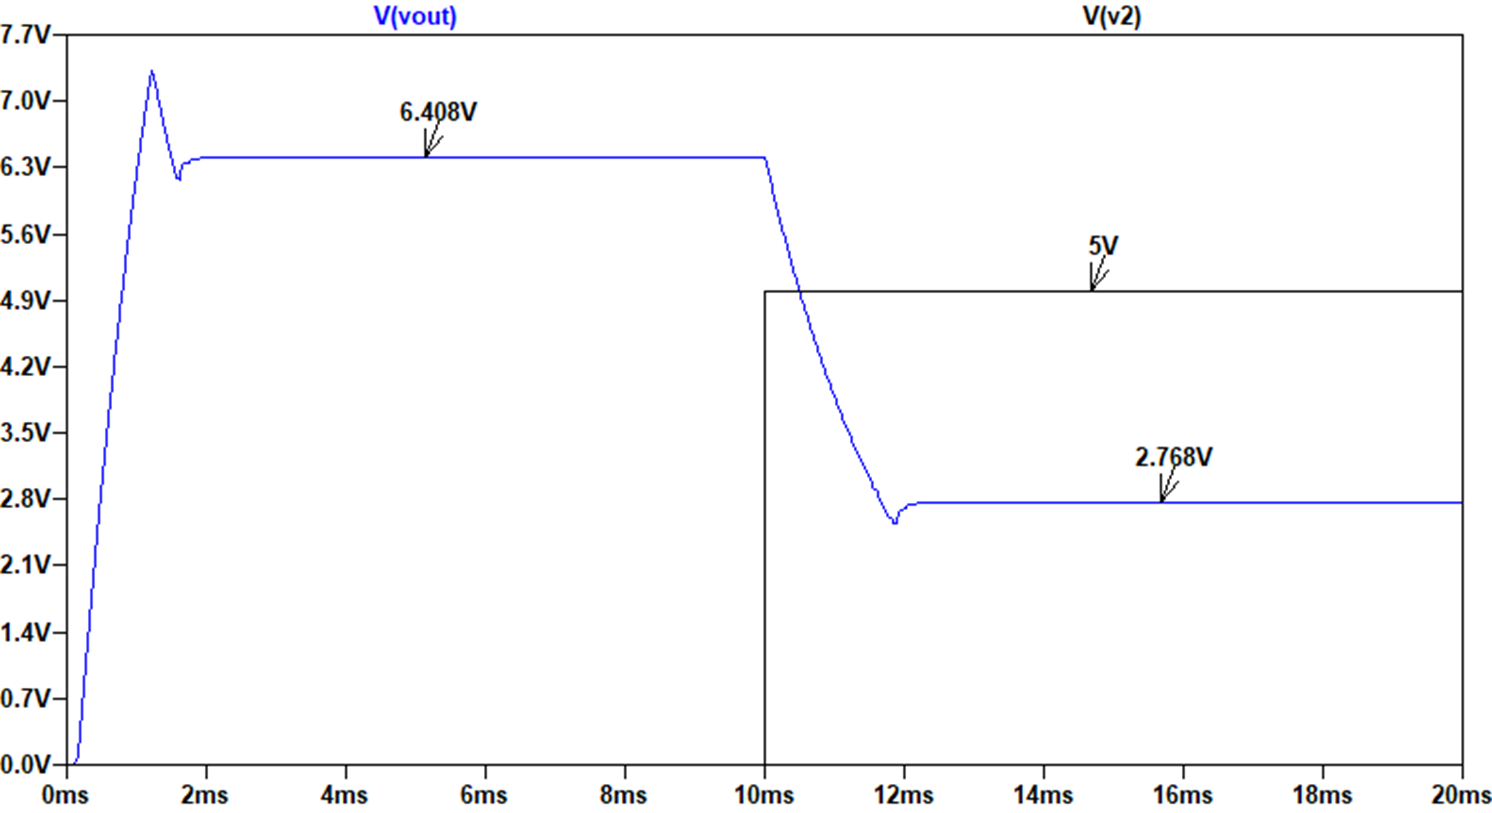
\includegraphics[scale=0.35]{imagenes/resultado_simulacion.png}
    \caption{Respuesta del convertidor (azul) contra el voltaje de control
            (negro).}
    \label{fig:sim_buck}
\end{figure}

En la figura \ref{fig:sim_buck} se muestra la respuesta del convertidor al
aplicar una señal escalón de $5\text{V}$ en la entrada de control. Se puede
observar que cuando el valor en el voltaje de control es de $0\text{V}$
la salida es de $6.408\text{V}$, además
cuando el valor del voltaje de control es de $5\text{V}$ el voltaje a la salida
del convertidor es de $2.768\text{V}$. Los cuales son valores cercanos a los esperados
al momento de realizar el diseño. 

Adicionalmente se puede observar que el rizado en el voltaje de salida del 
convertidor no es observable a la escala de voltaje en el que se está, esto debido
al uso de un valor más alto al calculado tanto para el inductor como para el 
capacitor del convertidor.

                                                                
\subsection{Prueba física del circuito}

Como último paso se realizó el diseño de un circuito impreso para probar el 
funcionamiento del circuito, en la figura \ref{fig:buck_pcb} se muestra la capa
superior e inferior del PCB.

\begin{figure}[H]
    \centering
    \begin{subfigure}{0.45\linewidth}
        \centering
        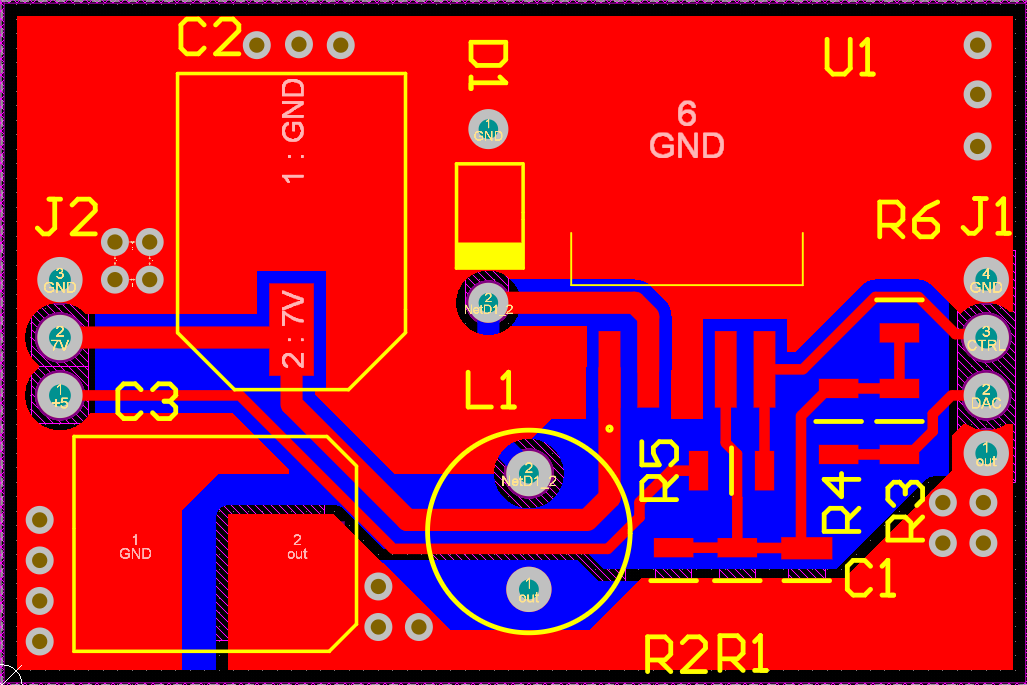
\includegraphics[scale=0.3]{imagenes/top_buck.png}
        \caption{Capa superior}
    \end{subfigure}
    \begin{subfigure}{0.45\linewidth}
        \centering
        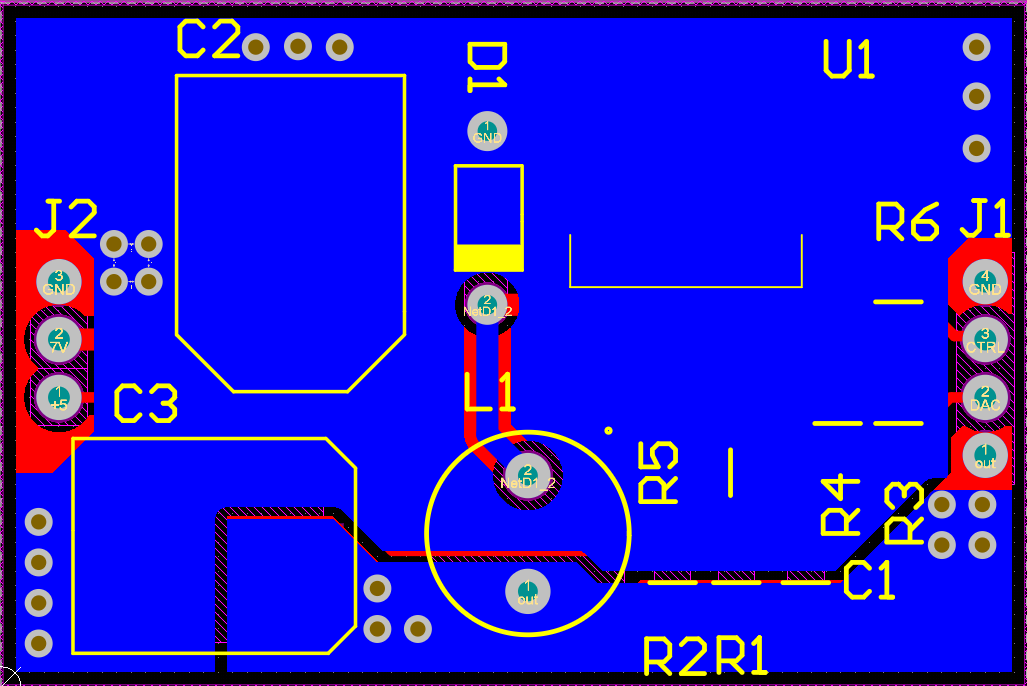
\includegraphics[scale=0.3]{imagenes/bottom_buck.png}
        \caption{Capa inferior}
    \end{subfigure}
    \vfill
    \begin{subfigure}{0.45\linewidth}
        \centering
        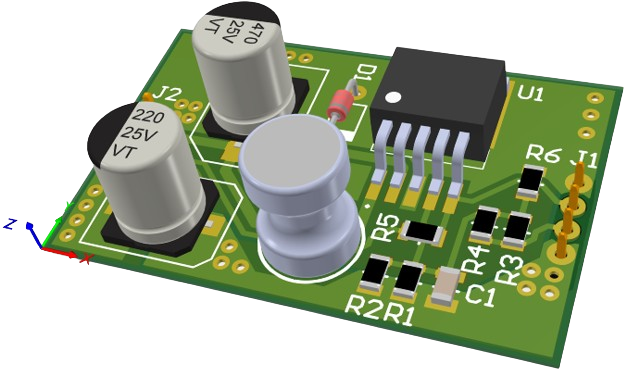
\includegraphics[scale=0.45]{imagenes/3d_buck.png}
        \caption{Vista 3D}
    \end{subfigure}
    \begin{subfigure}{0.45\linewidth}
        \centering
        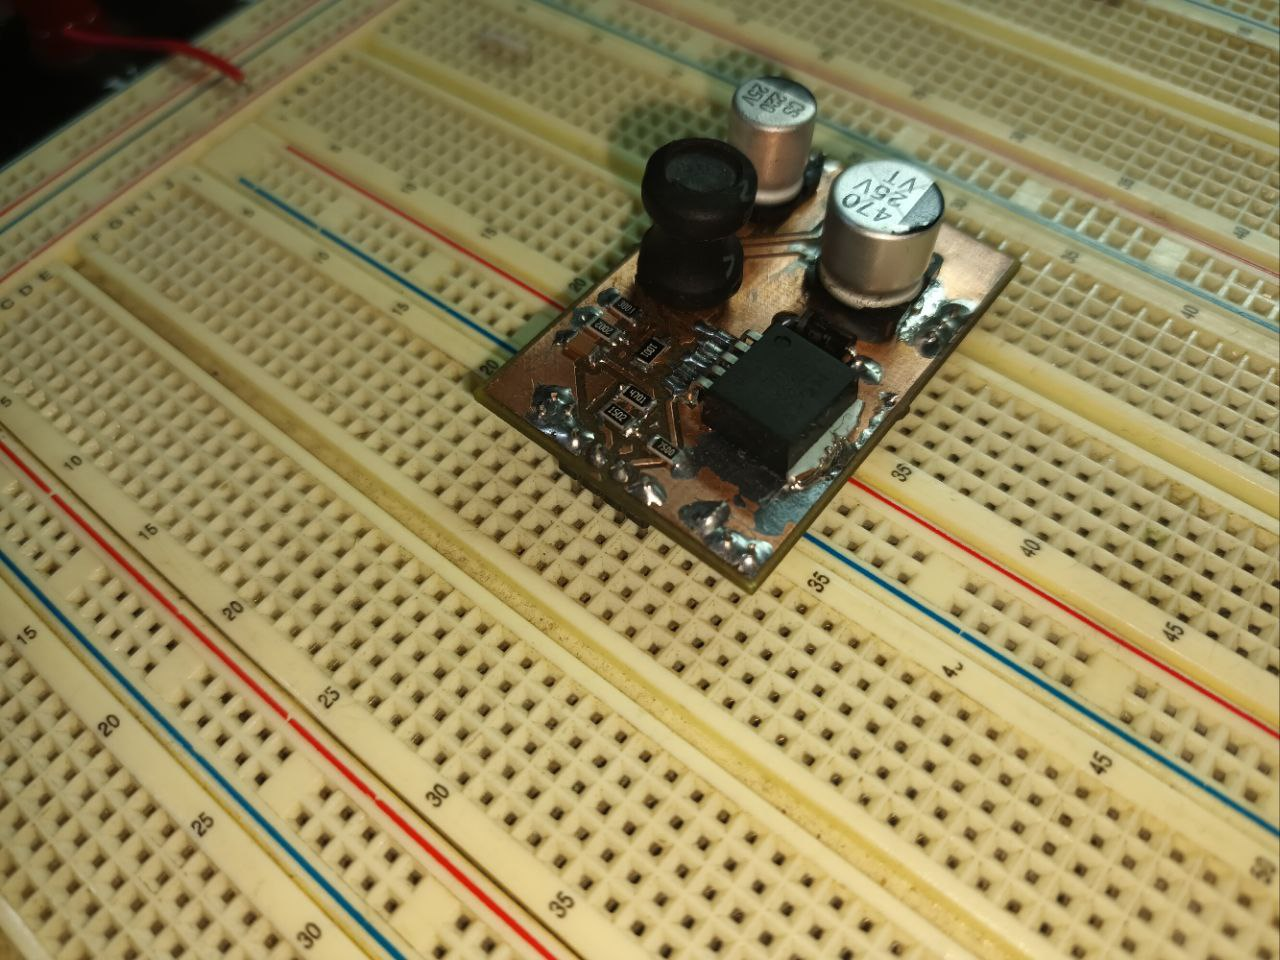
\includegraphics[scale=0.12]{imagenes/circuit_phis.jpg}
        \caption{PCB ensamblada}
    \end{subfigure}
    \caption{Diseño del PCB para el convertidor reductor}
    \label{fig:buck_pcb}
\end{figure}

Debido a que se manejan corrientes de hasta $1.5\text{A}$ es necesario que el
diseño del PCB sea capaz de manejar dicha corriente, para ello se empleó una 
calculadora de ancho de pistas \cite{noauthor_pcb_nodate}, con el cual se 
determinó que el ancho de las pistas debe ser de $0.53\text{mm}$ como mínimo,
esto tomando en cuenta que se estará usando un cobre con espesor de 1oz, y que
el maximo aumento de temperatura permitido es de 10\textordmasculine C. 

Se programó el microcontrolador ATmega328p para que genere una señal 
cuadrada de $5\text{V}$ con un periodo de 10 segundos en el pin PB1,
la cual se conectó a la entrada de control del convertidor. Al medir el voltaje
en la salida se obtuvo que el voltaje cuando se tienen $5\text{V}$ en la entrada
de control es de $2.76\text{V}$, mientras que cuando se tiene $0\text{V}$
en la entrada de control el voltaje a la salida es de $6.40\text{V}$, estos 
valores son cercanos a los esperados, por lo que el convertidor diseñado
funciona de forma correcta.

El circuito construido en protoboard para la prueba del convertidor se muestra
en la figura \ref{fig:prueba_buck}.

\begin{figure}[H]	
    \centering
    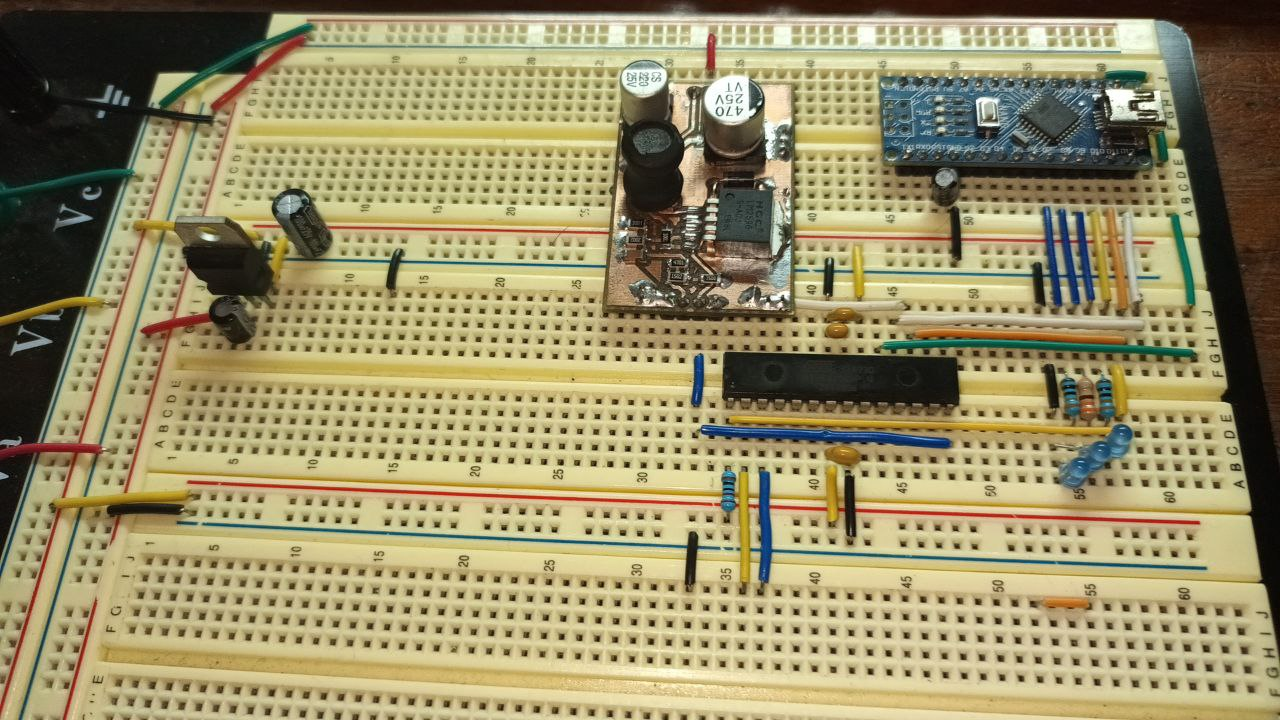
\includegraphics[scale=0.2]{imagenes/prueba_buck.jpg}
    \caption{Circuito para prueba del convertidor reductor (Arduino Nano únicamente
    es para programar el ATmega328p)} 
    \label{fig:prueba_buck}
\end{figure}

El código empleado en la prueba se muestra a continuación.

\begin{table}[H]
    \begin{lstlisting}
        #define F_CPU 8000000UL
        #include <avr/io.h>
        #include <util/delay.h>


        int main(void) {
                // ----     IO CONFIG  ---------
            DDRB = 0b00000011; // PB[7:2] input, PB1 out, PB0 out
            
            PORTB = 0b0000000; //activar PB0
            while (1) {
                PORTB |= 1<<1; //PB1 en 1
                _delay_ms(10000);
                PORTB &= ~(1<<1); //PB1 en 0
                _delay_ms(10000);
            }
        }

    \end{lstlisting}
    \caption{Código para prueba del convertidor reductor}
\end{table}

\section{Sensor de corriente}

    Para poder usar el convertidor reductor explicado en la sección
    \ref{sec:buck_design} es necesario medir la corriente que se
    está entregando a la batería. Para ello se diseñó un sensor de corriente
    basado en el amplificador operacional TL082.

    El sensor tiene 2 componentes principales, el amplificador diferencial y 
    la resistencia de sensado. El amplificador diferencial se encarga de 
    amplificar la diferencia de potencial entre los terminales de la resistencia
    de sensado, la cual es proporcional a la corriente que circula por la misma.
    La resistencia de sensado tiene un valor de $15 \text{m}\Omega$, con una
     tolerancia de $\pm 5\%$.

    Para poder medir una corriente máxima de $1.5\text{A}$ se escogió que 
    la ganancia para el amplificador diferencial (ver figura \ref{fig:ampDif})
    sea de $200\text{V/V}$, por lo que la salida del sensor será de
    $4.5\text{V}$ cuando la corriente sea de $1.5\text{A}$. Para obtener
    la ganancia deseada, se calcularon los valores de resistencia 
    necesarios utilizando la Ecuación \ref{eq:ampDifSimp}, fijando 
    el valor de $R_2$ en
    $1.5\text{K}\Omega$, obteniendo que el valor de $R_4$ debe ser de 
    $300\text{K}\Omega$. Debido a la  simplificación del circuito hecha en la 
    sección \ref{sec:ampDif} el valor de $R_1$ debe ser de $1.5\text{K}\Omega$
    y el valor de $R_3$ debe ser de $300\text{K}\Omega$. El sensor de corriente 
    diseñado se muestra en la figura \ref{fig:sensor_corriente}.

    \begin{figure}[H]
        \centering
        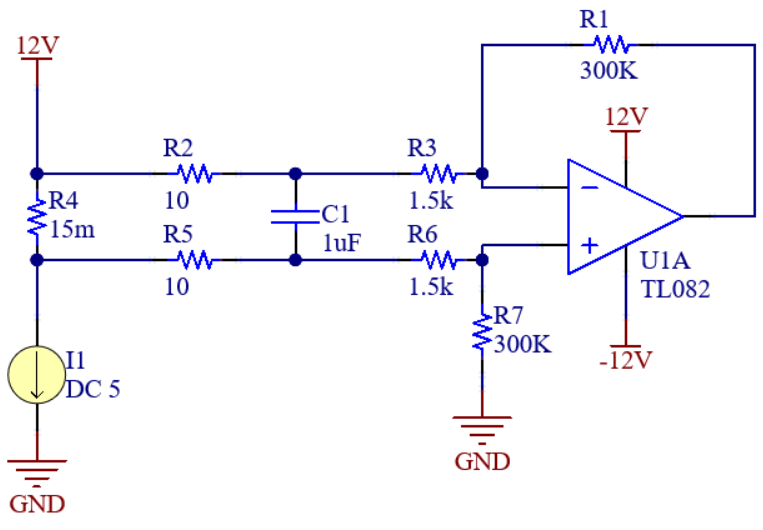
\includegraphics[scale=0.5]{imagenes/current_sensor.png}
        \caption{Sensor de corriente diseñado}
        \label{fig:sensor_corriente}
    \end{figure}

    con lo explicado anteriormente, el sensor tiene una ganancia final de 
    $3\text{V/A}$, la ecuación \ref{eq:sensor} describe la relación entre
    la corriente que circula por la resistencia de sensado y el voltaje de salida
    del amplificador diferencial.

    \begin{equation}
        V_{out} = 3I_1
        \label{eq:sensor}
    \end{equation}
    
    Para la alimentación del sensor es necesario un mínimo de $\pm7\text{V}$ en
    los pines de alimentación del amplificador operacional TL082, esto por dos 
    motivos, el primero es que el voltaje de salida del sensor es de $4.5\text{V}$
    cuando la corriente es de $1.5\text{A}$ tomando en cuenta que este opamp 
    no es del tipo \textit{rail to rail}, por lo que el voltaje de salida no
    puede ser igual al voltaje de alimentación, y el segundo motivo es que el
    voltaje en modo común de este amplificador tiene como limite superior el
    voltaje de alimentación positivo, por lo que es necesario que el voltaje 
    de alimentación sea mayor que el voltaje máximo de que recibirá en sus entradas,
    que para este caso es de $6.4\text{V}$. Para alimentar el sensor se empleó
    una alimentación simétrica de $\pm 12\text{V}$.
    
    \subsection{Mediciones del Sensor de corriente}

    Para comprobar el correcto funcionamiento del sensor de corriente diseñado
    se realizaron mediciones para varios niveles de corriente. Para ello se
    empleó una fuente de voltaje simétrica a $\pm7\text{V}$, y se utilizaron resistencias de entre 
    $4\Omega$ y $30\Omega$ para simular la carga de la batería. Los resultados 
    obtenidos son mostrados en el cuadro \ref{tb:mediciones_sensor}. 

\begin{table}[H]
    \centering
    \begin{tabular}{|c|c|c|c|}
        \hline
    Corriente medida & Salida del sensor (V) & Valor Ideal (V) & Error (\%) \\
    \hline
    0.241            & 0.815                 & 0.795           & 2.48       \\
    0.480            & 1.546                 & 1584            & 2.40       \\
    0.713            & 2.270                 & 2.353           & 3.52       \\
    0.933            & 2.945                 & 3.079           & 4.35       \\
    1.143            & 3.592                 & 3.772           & 4.77       \\
    1.354            & 4.24                  & 4.47            & 5.11       \\
    1.564            & 4.88                  & 5.16            & 5.43 \\
     \hline     
    \end{tabular}

    \caption{Valores de salida del sensor de corriente diseñado}
    \label{tb:mediciones_sensor}
    \end{table}


    En la figura \ref{fig:mediciones_sensor} se muestra el circuito construido
    en protoboard para la medición de los valores presentados anteriormente.

    \begin{figure}[H]
        \centering
        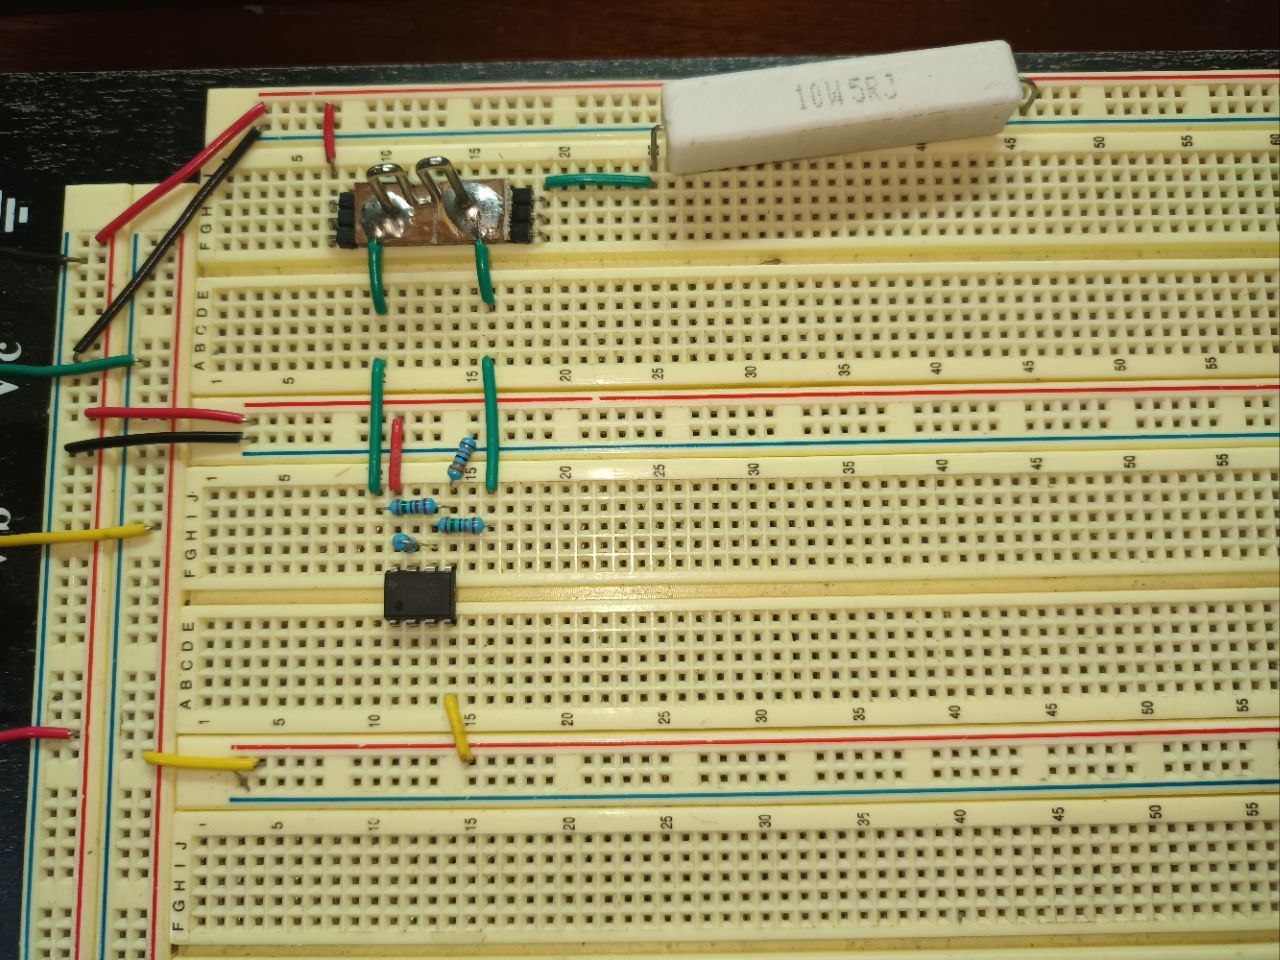
\includegraphics[scale=0.2]{imagenes/prueba_sensor.jpg}
        \caption{Circuito para medición del sensor de corriente}
        \label{fig:mediciones_sensor}
    \end{figure}


\section{Conversor digital a analógico (DAC)}

    Para controlar el voltaje de salida del convertidor reductor es necesario
    poder generar un voltaje de control de forma digital. Para ello se diseñó
    un conversor digital a analógico (DAC) utilizando un filtro RC de primer
    orden y un amplificador operacional en modo seguidor de voltaje. El DAC
    propuesto se muestra en la figura \ref{fig:dac}.

    \begin{figure}[H]
        \centering
        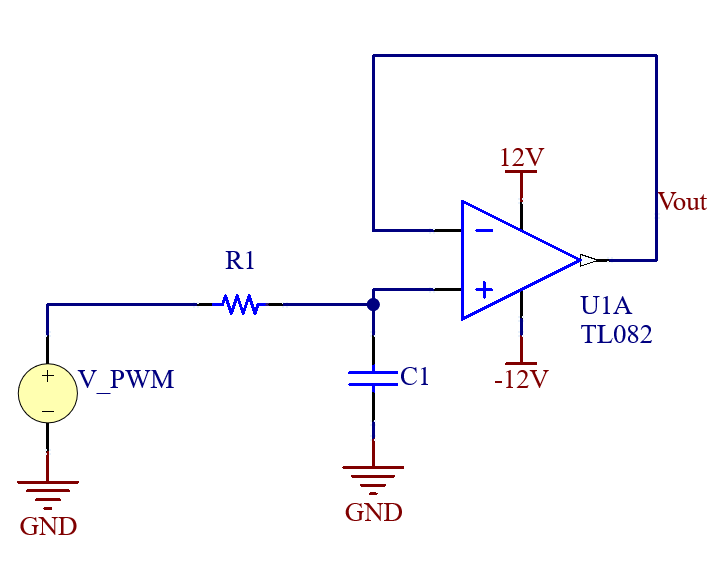
\includegraphics[scale=0.5]{imagenes/dac_disenio.png}
        \caption{DAC propuesto}
        \label{fig:dac}
    \end{figure}

    Ya que para la generación de la de PWM se utilizó el módulo PWM1 (debido
    a que este es el que presenta una mayor resolución) del ATmega328p, con el 
    cual se puede generar una señal PWM con una resolución de 10 bits, que en
    conjunto con una frecuencia de operación para el microcontrolador de $8\text{MHz}$
    se obtiene una frecuencia de PWM de $7.81\text{KHz}$, se determinó que la 
    frecuencia de corte del filtro RC sea de $70\text{Hz}$, de forma el armónico
    de mayor magnitud (el cual es el de frecuencia $7.81\text{KHz}$) sea atenuado
    en $-40\text{dB}$. 

    La frecuencia de corte para el filtro RC está dada por la ecuación \ref{eq:fc_dac},
    donde $R$ es el valor de la resistencia y $C$ es el valor del capacitor, mostrados
    en la figura \ref{fig:dac}.

    \begin{equation}
        f_c = \frac{1}{2\pi RC}
        \label{eq:fc_dac}
    \end{equation}

    Se fijó el valor del capacitor en $0.1\mu\text{F}$, por lo que el valor de la
    resistencia es de $22.7\text{K}\Omega$, por lo que se utilizará el valor 
    de resistencia comercial más cercano, el cual es de $22\text{K}\Omega$.
    Este cambio realizado en valor de la resistencia no afecta
    significativamente el comportamiento del filtro, ya que el objetivo 
    principal del mismo es atenuar los armónicos de la señal PWM, que es 
    dos órdenes de magnitud mayor a la frecuencia de corte del filtro.

    \subsection{Simulación del DAC}

    Para comprobar el correcto funcionamiento del DAC diseñado se realizó una
    simulación del mismo. Para ello se empleó el simulador LTspice, junto con
    el modelo spice proporcionado por texas instruments para el circuito integrado
    TL082 (descarga disponible en \cite{noauthor_tl082_nodate}). Para ello se 
    generó una señal pwm de $15.625KHz$ la cual varía su ciclo de trabajo 
    de forma que en la salida se obtenga una señal senoidal de $10\text{Hz}$. 
    En la figura
    \ref{fig:sim_dac} se muestra la respuesta del DAC ante la señal PWM de entrada.

    \begin{figure}[H]
        \centering
        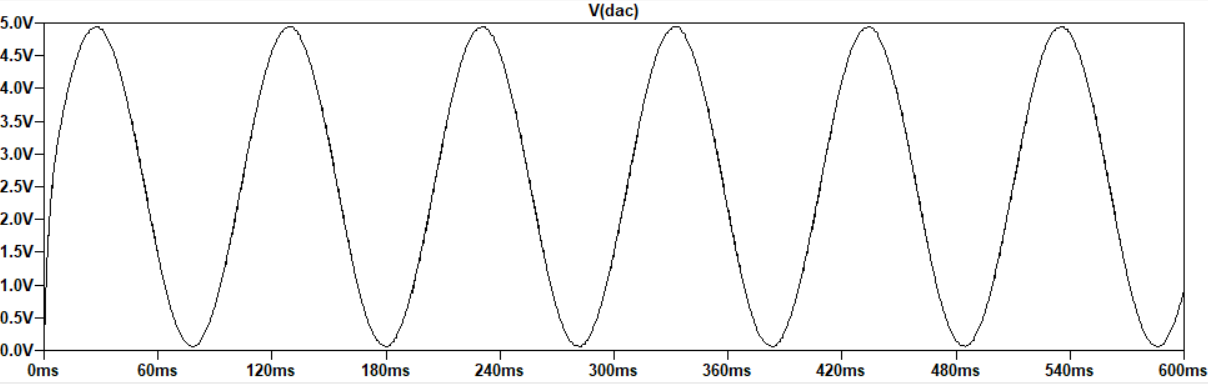
\includegraphics[scale=0.45]{imagenes/dac_out.png}
        \caption{Respuesta del DAC ante una señal PWM}
        \label{fig:sim_dac}
    \end{figure}

    En la figura \ref{fig:sim_dac} se puede observar que la señal de salida
    del DAC es una señal senoidal de $10\text{Hz}$, que es lo esperado ya 
    que la señal PWM varía su ciclo de trabajo también de forma senoidal.
    Además, se puede observar que el valor máximo de la señal de salida es
    de $5\text{V}$, mientras que el valor mínimo es cercano $0\text{V}$
    comprobando que el DAC funciona de forma correcta, ya que la señal PWM
    varía su ciclo de trabajo entre $0\%$ y $100\%$, haciendo que el valor 
    DC de la señal PWM varíe también entre $0\text{V}$ y $5\text{V}$.

    Adicionalmente en las figuras \ref{fig:sim_dac_fft} y \ref{fig:sim_dac_fft_in}
    se muestra la transformada de Fourier discreta (DFT) de la señal de salida
    del DAC, y de la señal PWM de entrada respectivamente. Se puede ver 
    que los armónicos correspondientes a la señal PWM de entrada son atenuados
    hasta el punto de que no son visibles en la DFT de la señal de salida del
    DAC, lo cual es lo esperado, ya que el filtro RC tiene una frecuencia de corte
    de $72\text{Hz}$, mientras que la frecuencia de la señal PWM es de 
    $15.625\text{KHz}$.

    \begin{figure}[H]
        \centering
        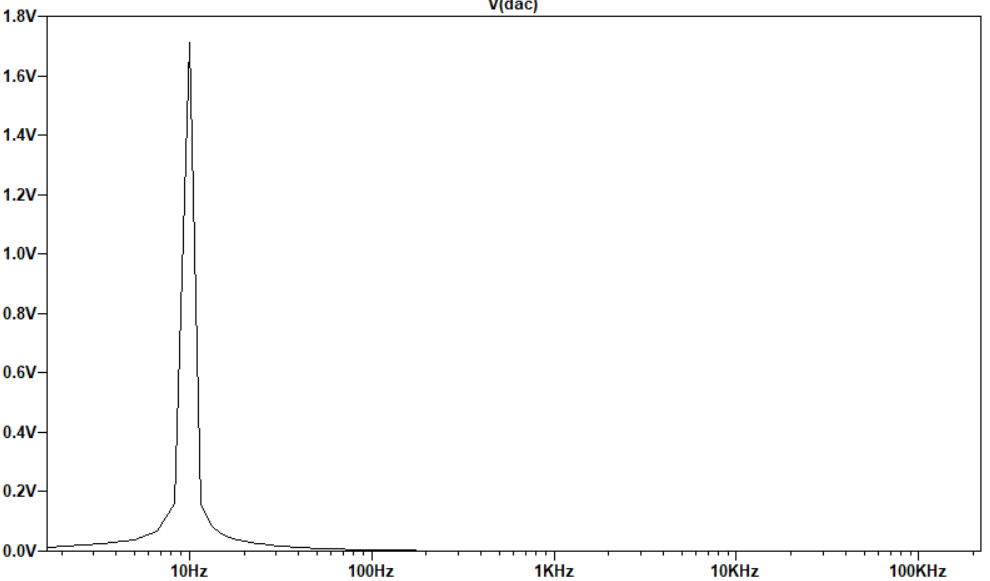
\includegraphics[scale=0.45]{imagenes/fft_dac_salida.png}
        \caption{DFT de la señal de salida del DAC}
        \label{fig:sim_dac_fft}
    \end{figure}

    \begin{figure}[H]
        \centering
        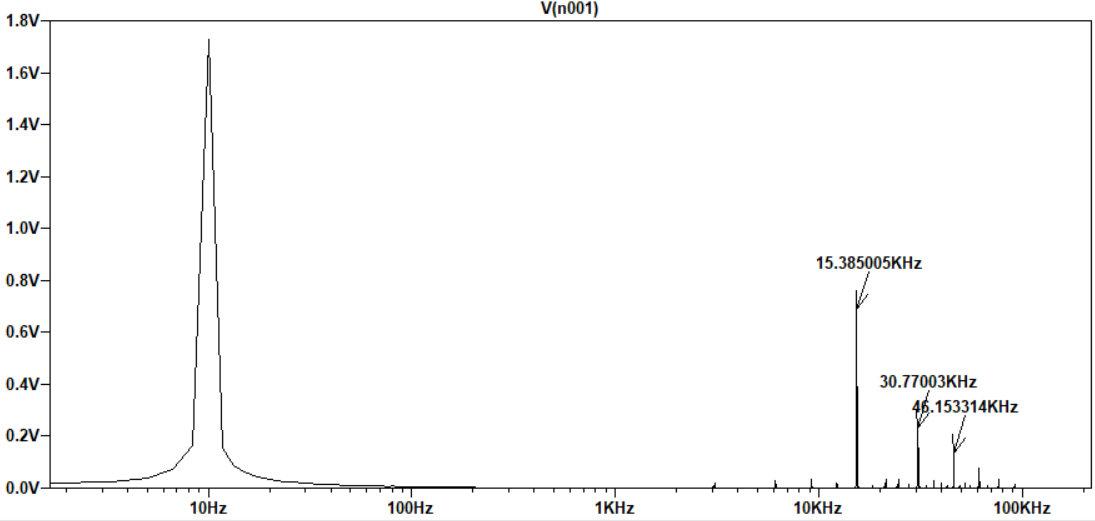
\includegraphics[scale=0.45]{imagenes/fft_dac_pwm.png}
        \caption{DFT de la señal PWM de entrada}
        \label{fig:sim_dac_fft_in}
    \end{figure}


    \subsection{Prueba física del DAC}

    Por último, se armó el circuito diseñado para comprobar
    el correcto funcionamiento del DAC. Para ello se utilizó un microcontrolador
    ATmega328p programado para generar una señal PWM de $15.625\text{KHz}$,
    a la cual se le varió el ciclo de trabajo de forma que en la salida del DAC
    se obtuviera una señal senoidal, el código empleado se encuentra en
    el anexo \ref{sec:codigo_dac}. En la figura \ref{fig:prueba_dac} se muestra
    el circuito armado en protoboard para la prueba del DAC.




    \section{Multiplicador de Voltaje}

    Debido a que el sensor de corriente y el DAC diseñados necesitan una
    alimentación simétrica de $\pm 7\text{V}$ (como mínimo), se diseñó 
    un multiplicador de voltaje basado en el circuito \textit{negative 
    Dickson charge pump} presentado en la sección \ref{sec:charge_pump}.


    Puesto que este necesita de una señal cuadrada, se utilizó un inversor
    elaborado con un transistor BJT , en cascada con una etapa de salida 
    \textit{push-pull}. El inversor es empleado para generar una señal
    cuadrada de amplitud $12\text{V}$ a partir de una señal cuadrada 
    de $5\text{V}$, mientras que la etapa \textit{push-pull}
    es utilizada para aumentar la corriente de salida del inversor, de forma
    que sea capaz de alimentar el multiplicador de voltaje. El circuito
    se muestra en la figura \ref{fig:inversor}.
    
    \begin{figure}[H]
        \centering
        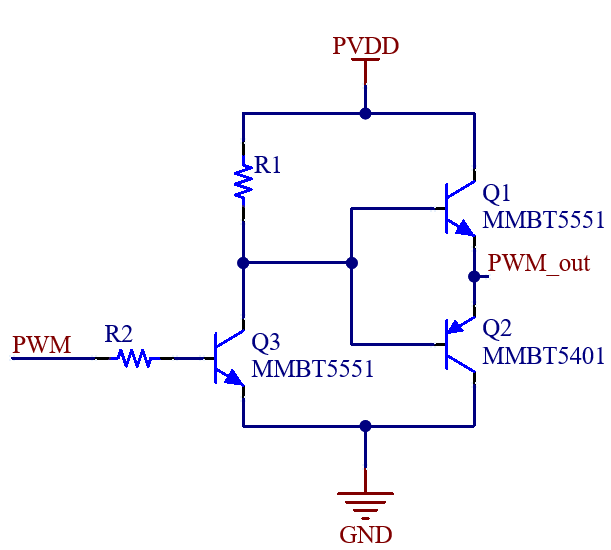
\includegraphics[scale=0.5]{imagenes/clk_gen.png}
        \caption{Inversor utilizado para generar la señal cuadrada}
        \label{fig:inversor}
    \end{figure}

    Para determinar los valores de $R_1$ y $R_2$
    se asumió que el voltaje entre base y emisor ($v_{be}$) del transistor $Q_3$
    es de $1\text{V}$  y que la ganancia en corriente del 
    transistor $Q_3$ es de $10$ \cite{mmtb5551}. Con lo anterior, se fijó el 
    valor de $R_2$ en $1\text{K}\Omega$, por 
    lo que la corriente en la base de $Q_3$ es de $I_b = 4\text{mA}$, y el valor
     esperado para la corriente de colector es de $I_c = 40\text{mA}$.

    Para que este transistor actúe como un inversor es necesario que 
    el transistor $Q_3$ se encuentre alternando entre
    las regiones de corte y saturación. Para ello es necesario
    que el producto $I_cR_1$ sea mayor al voltaje en el nodo PVDD, el cual
    es de $12\text{V}$:
    
    $$
        I_cR_1 > 12\text{V}
    $$
    
   
    $$
        R_1 > \frac{12\text{V}}{40\text{mA}} = 300 \Omega
    $$

    
    Por lo que se utilizó un valor de $R_1 = 1\text{K}\Omega$. Esta señal es 
    pasada en la etapa \textit{push-pull} para aumentar la corriente de salida
    del inversor,asi como disminuir la impedancia, de forma que sea 
    capaz de alimentar el multiplicador de voltaje.

    Para el diseño del multiplicador de voltaje se estableció que la 
    el valor de $C_1$ y $C_2$ sea de
    $1\mu\text{F}$, que el valor de salida requerido debe ser menor o igual
    a $-7\text{V}$ y el número de etapas($N$) es igual a 1. En la 
    ecuación \ref{eq:dickson_charge_neg}  se toma en cuenta la
    capacitancia parásita de los diodos ($C_s$), para el diseño se asumió
    que estas capacitancias no son significativas en comparación con 
    $C_1$ y $C_2$,por lo que se asume $C_s = 0$.
    Con lo anterior, la ecuación \ref{eq:charge_pump} se simplifica a la
    ecuación \ref{eq:charge_pump_simp}. En la figura \ref{fig:charge_pump_dis}
    se muestra el circuito diseñado.

    \begin{figure}[H]
        \centering
        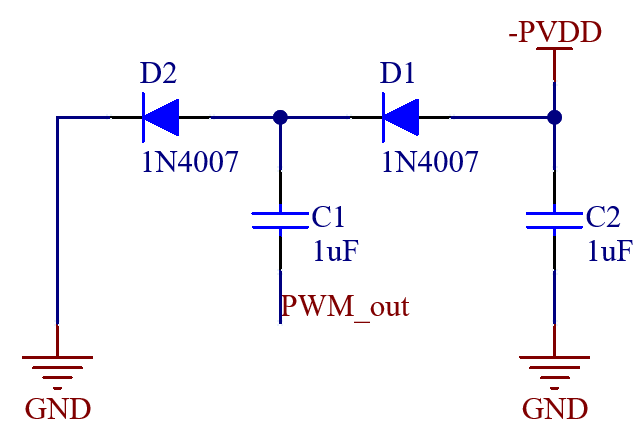
\includegraphics[scale=0.5]{imagenes/dickson_charge.png}
        \caption{Circuito diseñado para el multiplicador de voltaje}
        \label{fig:charge_pump_dis}
    \end{figure}

    \begin{equation}
        V_{out} = -\left(V_\Phi - V_D - \frac{I_{out}}{Cf}  \right)
        \label{eq:charge_pump_simp}
    \end{equation}

    Para determinar la frecuencia de operación, se utilizó la ecuación 
    \ref{eq:charge_pump_simp}, junto con la desigualdad 
    $V_{out} \leq -7\text{V}$, obteniendo la ecuación 
    \ref{eq:charge_pump_simp2}.

    \begin{equation}
        -\left(V_\Phi - V_D - \frac{I_{out}}{Cf}\right) \leq -7\text{V}
        \label{eq:charge_pump_simp2}    
    \end{equation}

    Para la amplitud de la señal cuadrada se utilizó el valor de 
    $V_\Phi = 12 \text{V}$, mientras que para 
    el valor de $V_D$ se utilizó el valor de $0.7\text{V}$, y se estimó que
    la corriente de salida del multiplicador de voltaje es de $10\text{mA}$.
    Despejando para la frecuencia se obtiene la ecuación \ref{eq:charge_pump_simp3}.

    \begin{equation}
        f \geq \frac{I_{out}}{C(V_\Phi - V_D - V_{out})}
        \label{eq:charge_pump_simp3}
    \end{equation}

    Reemplazando los valores en la ecuación \ref{eq:charge_pump_simp3} se obtiene
    la frecuencia de operación del multiplicador de voltaje debe de ser 

        $$
            f \geq \frac{10\text{mA}}{1\mu\text{F}(12\text{V} - 0.7\text{V}
             - 7\text{V})} \approx 2.325\text{KHz}
        $$

    Ya que este es un valor mínimo para la frecuencia de operación, al utilizar
    una frecuencia mayor se obtendrá un voltaje de salida mayor, por lo que se
    utilizó una frecuencia de operación de $7.81\text{KHz}$, la cual es la
    frecuencia de la señal PWM generada por el microcontrolador. 

    

    \section{Controlador}

    Para la gestión de los multiplexores de potencia y el control del convertidor
    reductor se diseñó un controlador basado en el microcontrolador ATmega328p.
    El cual tiene las siguientes funciones:

    \begin{itemize}
        \item Controlar el voltaje y corriente de salida del convertidor reductor
        \item Controlar que batería se está cargando mediante un multiplexor de potencia
        \item Controlar el multiplexor de potencia para seleccionar la batería
        que proporcionará la alimentación al agente robótico.
        \item Permitir la comunicación con la estación de carga mediante comunicación
        UART.
        \item  Permitir la comunicación con el adaptador wifi mediante comunicación
        I2C.
        \item índicar de forma visual el estado de carga de las baterías mediante
        2 LEDs.
    \end{itemize}


    \section{Placa de expansión para el agente robótico}

        Luego de haber probado todos los sistemas en conjunto se procedió a diseñar
        una placa de expansión para el agente robótico Pololu 3Pi+ que permita
        la conexión de todos los sistemas diseñados. Para permitir la conexión
         entre ambas placas se utilizaron conectores 
        macho ubicados según los planos proporcionados por la 
        empresa Pololu \cite{noauthor_pololu_nodate}.
        Los pines utilizados para la comunicación o transmisión de potencia entre
        ambas placas son los siguientes:

        \begin{itemize}
            \item GND: Todos los pines etiquetados como GND en la placa de control
            del agente robótico son conectados con la tierra de la placa de expansión.
            \item VBAT: Este pin es utilizado para realizar la carga de las baterías
            NiMH presentes en el agente robótico.
            \item VSW: Este pin es utilizado para alimentar la placa de 
            control del agente robótico, al momento de que la batería NiMH 
            se encuentre descargada.

        \end{itemize}

    
        


\chapter{Estación de carga}

La estación de carga está compuesta por 2 partes, la primera es un circuito impreso
en el cual se encuentran los conectores USB, para la transmisión de potencia y 
datos entre la estación de carga y el sistema de carga multiquímica. La segunda
parte es una estructura impresa en 3D, la cual tiene como función principal
proveer un espacio para colocar el circuito impreso descrito anteriormente y 
los cables USB magnéticos que se utilizarán para realizar la conexión entre
la estación de carga y el sistema de carga multiquímica.


\section{Circuito impreso}

El circuito impreso tiene 4 componentes principales que se listan a continuación:

\begin{itemize}
    \item Conectores USB tipo A hembra
    \item Cables USB para transmisión de potencia y datos
    \item \textit{Headers} macho para comunicación serial
    \item Bornera de 2 pines para alimentación de la estación de carga
\end{itemize}
El circuito impreso diseñado se muestra en la figura \ref{fig:pcb_estacion_carga}.

\begin{figure}[H]
    \centering
    \begin{subfigure}{0.9\linewidth}
        \centering
        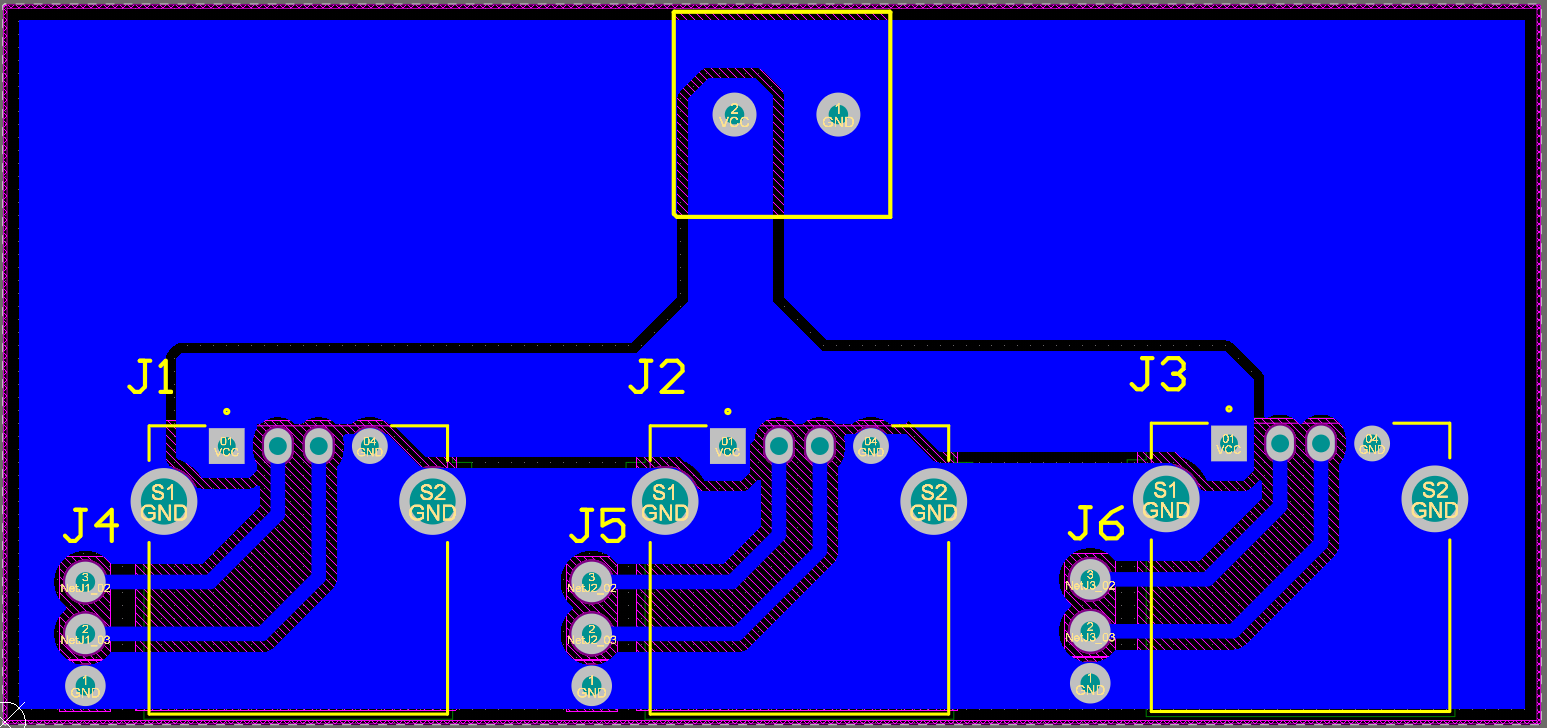
\includegraphics[scale=0.25]{imagenes/bottom_charging.png}
        \caption{Capa inferior}
    \end{subfigure}
    \vfill
    \begin{subfigure}{0.9\linewidth}
        \centering
        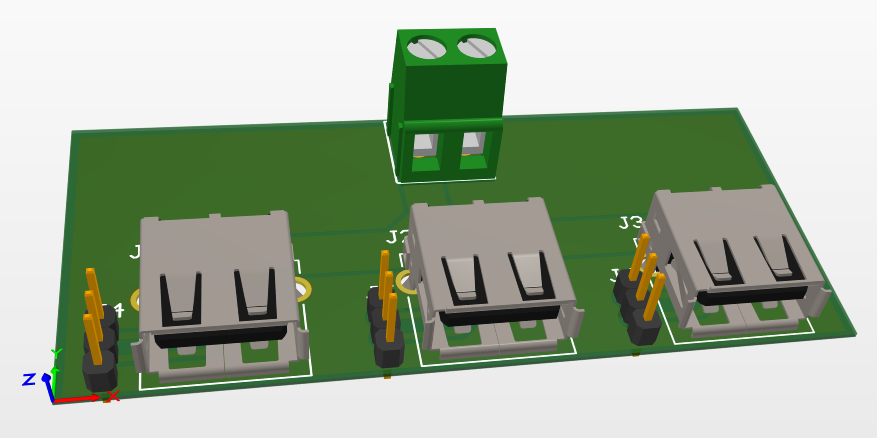
\includegraphics[scale=0.45]{imagenes/3d_charging.png}
        \caption{Vista 3D}
    \end{subfigure}
    \caption{Diseño del PCB para la estación de carga}
    \label{fig:pcb_estacion_carga}
\end{figure}

La PCB de la estación de carga soldada se muestra en la figura \ref{fig:pcb_estacion_carga_soldada}.

\begin{figure}[H]
    \centering
    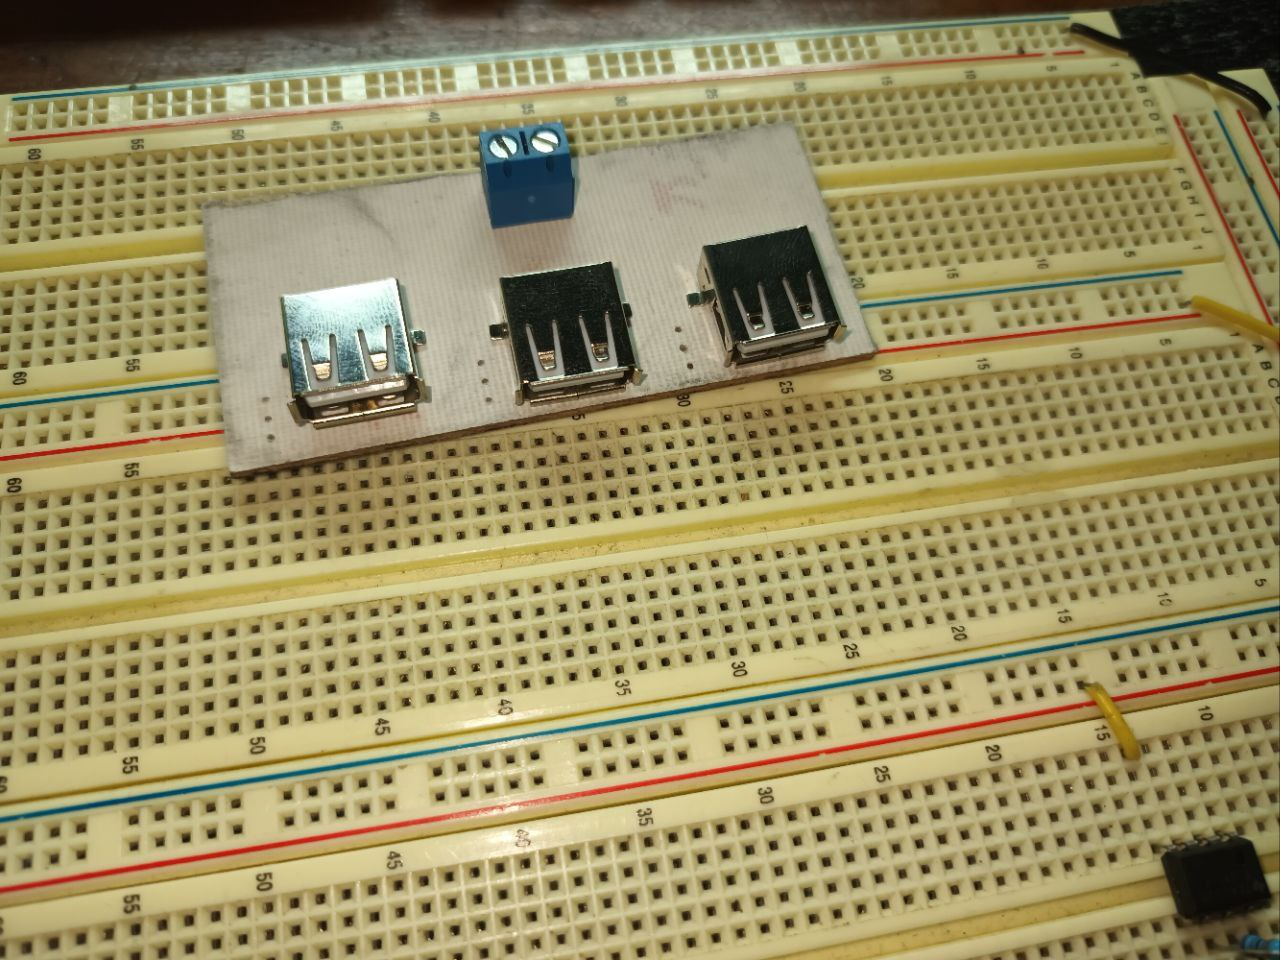
\includegraphics[scale=0.2]{imagenes/charger_pcb.jpg}
    \caption{PCB de la estación de carga soldada}
    \label{fig:pcb_estacion_carga_soldada}
\end{figure}
\fi

% CONCLUSIONES
% ------------------------------------------------------------------------------
\ifdefined\CAPconclusiones
	\newpage
	\chapter{Conclusiones}
	\ifdefined\parpordefecto
		\defaultparformat{k-conclusiones}
	\else
		
\begin{itemize}
    
    \item Se logró diseñar una placa de expansión para el agente robótico
    Pololu 3Pi+ que incorpora un sistema de carga multiquímica capaz de
    gestionar la recarga de baterías de iones de litio (Li-ion) y níquel-metalhidruro (NiMH).
    asi como poder realizar la conmutación mediante un multiplexor de 
    potencia, entre ambas baterías para la 
    alimentación del agente robótico.

    \item Se realizó el diseño y la construcción de una estación de carga
    que proporciona tanto el voltaje como la corriente requerida para el
    funcionamiento óptimo del sistema de carga multiquímica, asi como la
    comunicación con el sistema de carga mediante comunicación UART.


\end{itemize}
	\fi
\fi

% RECOMENDACIONES
% ------------------------------------------------------------------------------
\ifdefined\CAPrecomendaciones
	\newpage
	\chapter{Recomendaciones}
	\ifdefined\parpordefecto
		\defaultparformat{l-recomendaciones}
	\else
		\begin{itemize}
    \item Para tener una mejor precisión en la medición de la corriente, evitar el uso
    de fuentes de voltaje negativos y reducir el espacio utilizado por el
    circuito de medición de corriente,
    se recomienda utilizar una resistencia con una menor tolerancia en empaquetado SMD, así como un 
    circuito integrado dedicado para medir corriente como lo puede ser el INA219, 
    o el INA190 de Texas Instruments.

    \item Utilizar un microcontrolador que posea un periférico de comunicación USB nativo,
    para evitar el uso de conversores USB a UART y poder hacer la placa de expansión
    compatible con protocolos de carga rápida como lo es el USB \textit{Power Delivery}, o el
    \textit{Quick Charge} de Qualcomm

    \item Emplear un circuito integrado dedicado que realice la función de 
    convertidor digital a analógico, para reducir el espacio utilizado en la placa
    de expansión, así como mejorar la precisión de la señal de voltaje para el control
    del convertidor reducir.

\end{itemize}

	\fi
\fi

% BIBLIOGRAFÍA
% ------------------------------------------------------------------------------
\ifdefined\CAPbibliografia
	\newpage
    \cleardoublepage\phantomsection
	\chapter{\bibname}
    \printbibliography[heading=none]
\fi

% ANEXOS
% ------------------------------------------------------------------------------
\ifdefined\CAPanexos
	\newpage
	\chapter{Anexos}
	\ifdefined\parpordefecto
		\defaultparformat{n-anexos}
	\else
		\section{Diagrama esquemático de la placa de expansión}
\label{sec:anexo_esquematico}

\begin{figure}[H]
    \centering
    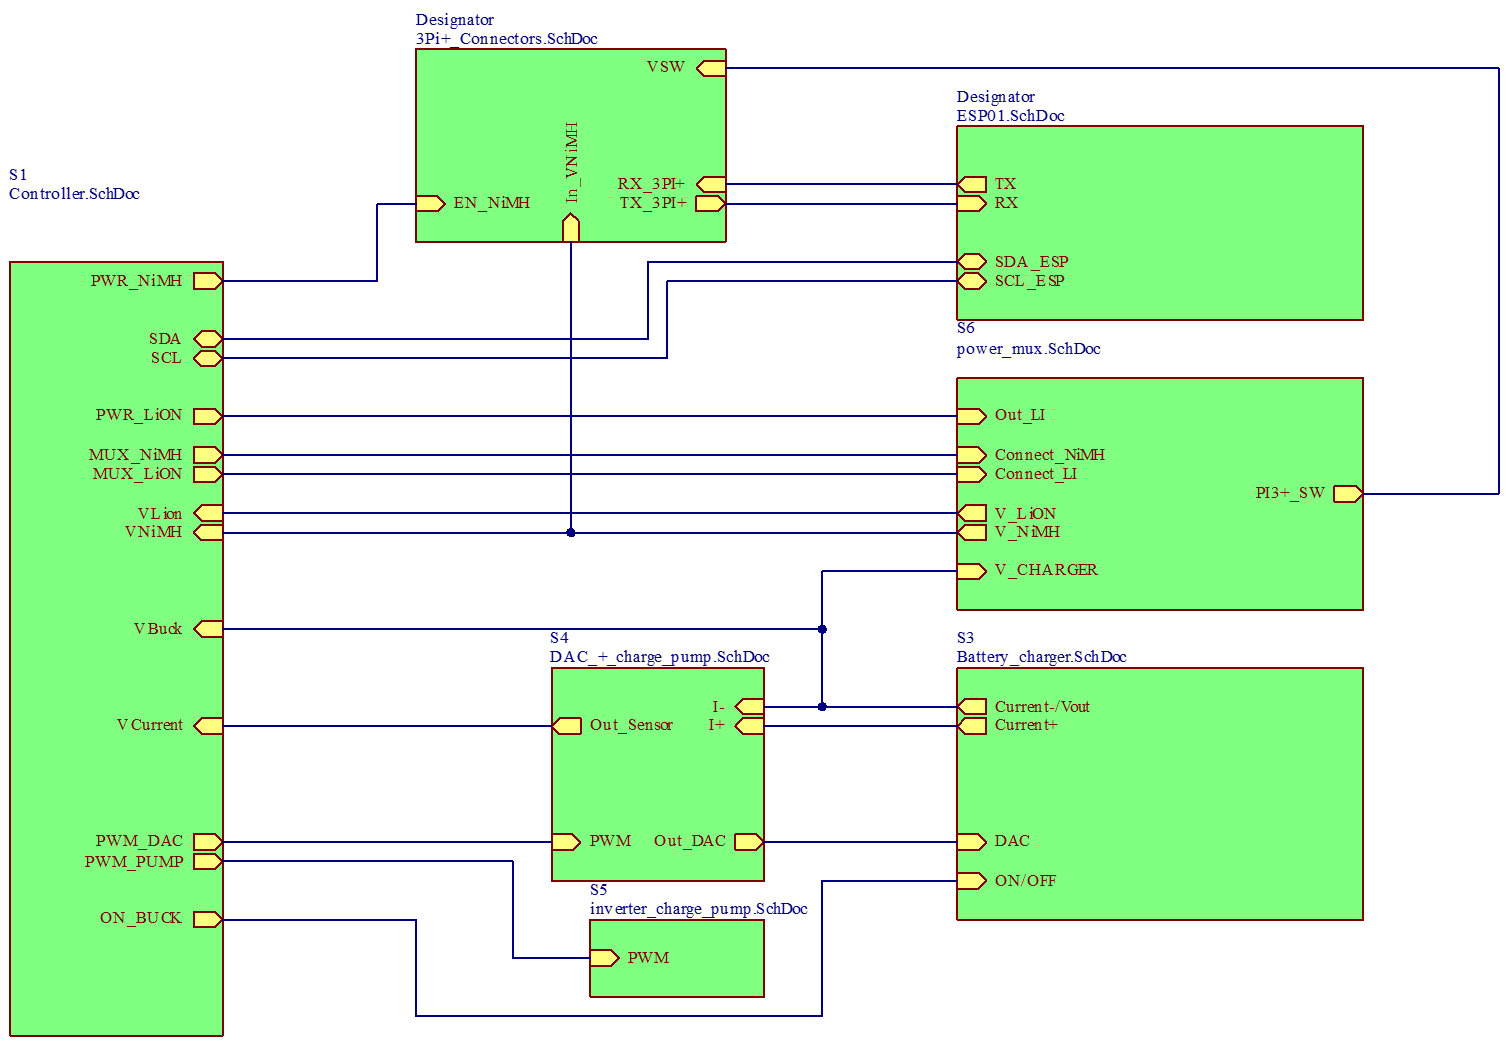
\includegraphics[scale=0.3]{imagenes/system_interconection.png}
    \caption{Interconexión de los circuitos en la placa de expansión}
    \label{fig:all}    
\end{figure}

\begin{figure}[H]
    \centering
    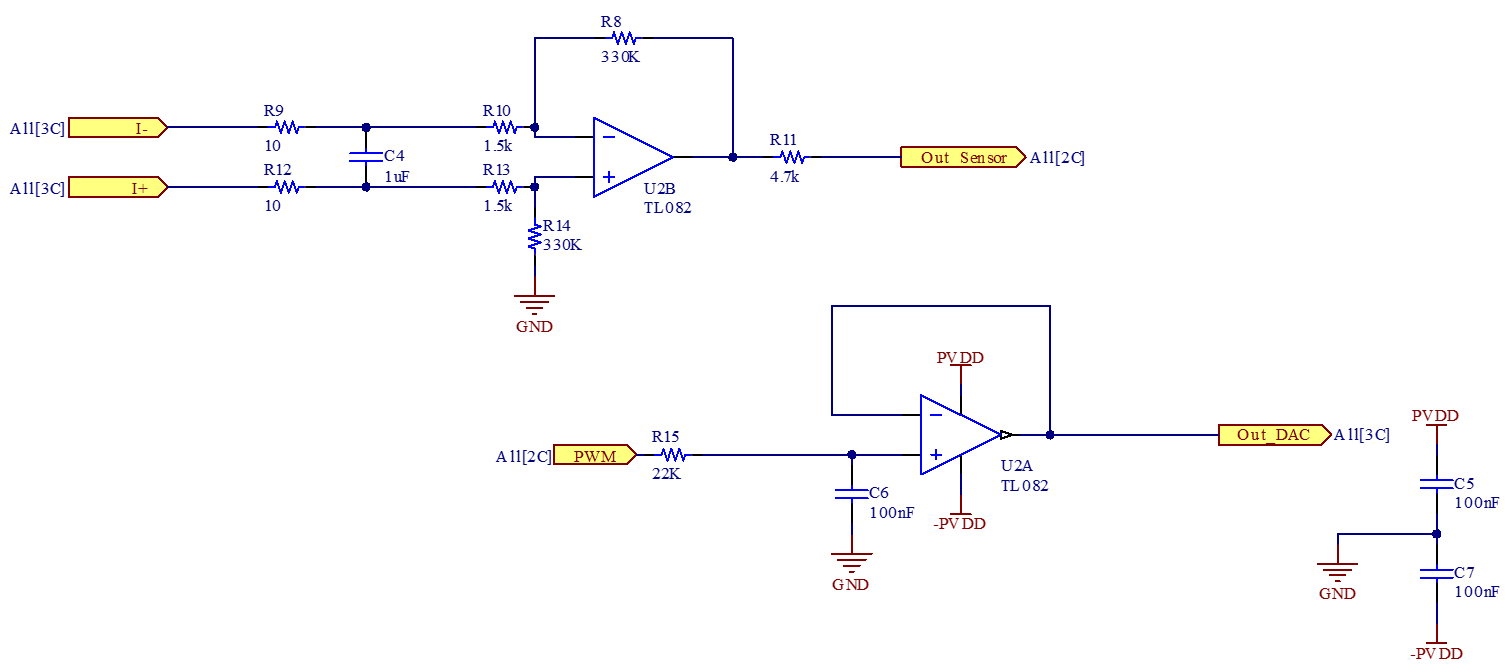
\includegraphics[scale=0.3]{imagenes/dac_sensor.png}
    \caption{Diagrama esquemático del sensor de corriente y el convertidor digital a analógico
    (S4 en la figura \ref{fig:all})}
    \label{fig:dac_sensor}
\end{figure}


\begin{figure}[H]
    \centering
    \includegraphics[scale=0.25]{imagenes/charge_pump.png}
    \caption{Diagrama esquemático del \textit{charge pump} (S5 en la figura \ref{fig:all})}
    \label{fig:charge_pump_anexo}
\end{figure}


\begin{figure}[H]
    \centering
    \includegraphics[scale=0.45]{imagenes/controlador_disenio.png}
    \caption{Diagrama esquemático del controlador (S1 en la figura \ref{fig:all})}
    \label{fig:controlador_anexo}
\end{figure}

\begin{figure}[H]
    \centering
    \includegraphics[scale=0.28]{imagenes/charger_anexos.png}
    \caption{Diagrama esquemático del convertidor reductor (S3 en la figura \ref{fig:all})}
    \label{fig:charger_anexo}
\end{figure}

\begin{figure}[H]
    \centering
    \includegraphics[scale=0.3]{imagenes/mux_anexo.png}
    \caption{Diagrama esquemático del multiplexor de potencia (S6 en la figura \ref{fig:all})}
    \label{fig:charger_anexo_mux}  
\end{figure}

\begin{figure}[H]
    \centering
    \includegraphics[scale=0.3]{imagenes/esp01.png}
    \caption{Diagrama esquemático del ESP01}
    \label{fig:esp01_anexo}
\end{figure}

\begin{figure}[H]
    \centering
    \includegraphics[scale=0.2]{imagenes/3pi+_anexo.png}
    \caption{Diagrama esquemático para los conectores del 3Pi+}
    \label{fig:3pi+_anexo}
\end{figure}

\section{Código fuente empleado en la prueba del DAC}

\label{sec:codigo_dac}

\lstinputlisting[style=atmega328]{../Charge_system_firmware/DAC_test.X/main.c}
\begin{table}[H]
    \caption{Código para prueba de funcionamiento del DAC}
\end{table}

\section{Código fuente empleado en la prueba de funcionamiento de la placa de expansión}
\label{sec:codigo_prueba_expansion}
\lstinputlisting[style=atmega328]{../Charge_system_firmware/Pololu_on_test.X/mian.c}
\begin{table}[H]
    \caption{Código para prueba de funcionamiento de la placa de expansión}
\end{table}

\section{Código fuente para el sistema de carga}
\label{sec:codigo_expansion}

\lstinputlisting[style=atmega328]{../Charge_system_firmware/Charging_system.X/main.c}
\begin{table}[H]
    \caption{Código para el sistema de carga}
\end{table}
	\fi
\fi

% GLOSARIO
% ------------------------------------------------------------------------------
\ifdefined\CAPglosario
	\newpage
	\printglossary
\fi

\end{document}